
\documentclass[preprint2]{emulateapj}

\usepackage{natbib}
\bibliographystyle{apj}
\usepackage{longtable}
\usepackage[]{graphicx}
\usepackage{amsmath}
\usepackage{natbib}
\usepackage{tabularx}
\usepackage{bm}
\usepackage{color}

%% Sometimes a paper's abstract is too long to fit on the
%% title page in preprint2 mode. When that is the case,
%% use the longabstract style option.

%% \documentclass[preprint2,longabstract]{aastex}

\newcommand{\vdag}{(v)^\dagger}
\newcommand{\myemail}{gsavorgn@astro.swin.edu.au}
\newcommand{\fitfigurewidth}{0.8\textwidth}


\shorttitle{M-M paper}
\shortauthors{Savorgnan et al.}

\begin{document}

\title{Supermassive black hole and host bulge affairs \\ II. The red and blue sequence in the $M_{\rm BH} - M_{\rm *,sph}$ diagram.}

%\author{G. A. D. Savorgnan\altaffilmark{1} and A. W. Graham\altaffilmark{1} and A. Marconi and E. Sani\altaffilmark{3} and L.K. Hunt}
%\affil{Centre for Astrophysics and Supercomputing, Swinburne University of Technology, Hawthorn, Victoria 3122, Australia.}
%\email{gsavorgn@astro.swin.edu.au}


\author{G. A. D. Savorgnan and A. W. Graham}
\affil{Centre for Astrophysics and Supercomputing, Swinburne University of Technology, Hawthorn, Victoria 3122, Australia.}
\email{gsavorgn@astro.swin.edu.au}
\author{A. Marconi}
\affil{Dipartimento di Fisica e Astronomia, Universit\'a di Firenze, via G. Sansone 1, I-50019 Sesto Fiorentino, Firenze, Italy.}
\and
\author{E. Sani}
\affil{European Southern Observatory, Alonso de Cordova, Vitacura 3107, Santiago, Chile.}

%\and

%\author{A. W. Graham\altaffilmark{1}}
%\affil{Centre for Astrophysics and Supercomputing, Swinburne University of Technology, Hawthorn, Victoria 3122, Australia.}

%% Notice that each of these authors has alternate affiliations, which
%% are identified by the \altaffilmark after each name.  Specify alternate
%% affiliation information with \altaffiltext, with one command per each
%% affiliation.

%\altaffiltext{1}{}
%\altaffiltext{2}{Society of Fellows, Harvard University.}
%\altaffiltext{3}{present address: Center for Astrophysics,
%    60 Garden Street, Cambridge, MA 02138}
%\altaffiltext{4}{Visiting Programmer, Space Telescope Science Institute}
%\altaffiltext{5}{Patron, Alonso's Bar and Grill}

%% Mark off your abstract in the ``abstract'' environment. In the manuscript
%% style, abstract will output a Received/Accepted line after the
%% title and affiliation information. No date will appear since the author
%% does not have this information. The dates will be filled in by the
%% editorial office after submission.

\begin{abstract}
In our first paper, we performed a detailed (i.e.~bulges, disks, bars, spiral arms, rings, haloes, nuclei, cores, etc.) 
decomposition of 66 galaxies, with directly measured black hole masses, 
that had been imaged at $3.6\rm~\mu m$ with \emph{Spitzer}.
Our sample is the largest to date and, for the first time, the decompositions were checked to be consistent with the galaxy kinematics.
Here we present correlations between the black hole mass, $M_{\rm BH}$, 
and the host spheroid (and galaxy) luminosity, $L_{\rm sph}$ (and $L_{\rm gal}$), 
and also stellar mass, $M_{\rm *,sph}$.
Most previous studies have used galaxy samples that were overwhelmingly dominated by high-mass, early-type objects.
Instead, our sample includes 17 spiral galaxies, half of which have $M_{\rm BH} < 10^7\rm~M_\odot$, 
and allows us to better investigate the poorly studied low-mass end of the $M_{\rm BH} - M_{\rm *,sph}$ correlation.
The bulges of early-type (E + S0) galaxies follow $M_{\rm BH} \propto M_{\rm *,sph}^{1.04 \pm 0.10}$, 
consistent with a dry-merging formation scenario,
and define a tight \emph{red sequence} with intrinsic scatter $\epsilon_{(Y|X)} = 0.43 \pm 0.06\rm~dex$.
On the other hand, the bulges of late-type (Sp) galaxies define a much steeper \emph{blue sequence}, 
with $M_{\rm BH} \propto M_{\rm *,sph}^{2-3}$, 
indicating that gas-rich processes feed the black hole more efficiently than the host bulge as they grow. 
We additionally report that: i) S\'ersic galaxies follow $M_{\rm BH} \propto M_{\rm *,sph}^{1.48 \pm 0.20}$, a less steep sequence than previously reported; 
ii) bulges with S\'ersic index $n_{\rm sph}<2$, argued by some to be pseudo-bulges, 
are not offset to lower $M_{\rm BH}$ from the correlation defined by bulges with $n_{\rm sph}>2$; 
and iii) $L_{\rm sph}$ and $L_{\rm gal}$ correlate equally well with $M_{\rm BH}$, in terms of intrinsic scatter, only for early-type galaxies; 
once reasonable numbers of spiral galaxies are included, the correlation with $L_{\rm sph}$ is better than that with $L_{\rm gal}$. {\bf 241 words} 

\end{abstract}

\keywords{\bf keywords}

\section{Introduction}
\label{sec:int}
A quarter of a century ago, 
\cite{dressler1989} foresaw a ``rough scaling of black hole mass with the mass of the spheroidal component'' of galaxies, 
as suggested by the sequence of five galaxies (M87, M104, M31, M32 and the Milky Way). 
\cite{yee1992} also announced a relation between what was effectively black hole mass and galaxy mass for bright early-type galaxies.
This ``rough scaling'' was a premature version of the nowadays popular correlation between black hole mass, $M_{\rm BH}$,  
and host spheroid luminosity, $L_{\rm sph}$, and also host spheroid mass, $M_{\rm sph}$ 
\citep{kormendyrichstone1995,magorrian1998,marconihunt2003,haringrix2004}. 
These early studies were dominated by high-mass, early-type galaxies, 
for which they reported a quasi-linear $M_{\rm BH} - M_{\rm sph}$ relation, 
consistent with a dry-merging formation scenario which would build and maintain a linear scaling. 
Subsequent studies of the $M_{\rm BH} - L_{\rm sph}$ and $M_{\rm BH} - M_{\rm sph}$ diagrams 
(\citealt{ferrareseford2005,lauer2007,graham2007,gultelkin2009,sani2011,beifiori2012,erwingadotti2012,
vika2012,vandenbosch2012,mcconnellma2013,kormendyho2013,rusli2013}; 
see \citealt{graham2015bulges} for an extensive review about the early discovery and successive improvements of these correlations)
continued to use galaxy samples dominated by high-mass, early-type systems having $M_{\rm BH} \gtrsim 0.5 \times 10^8~\rm M_\odot$, 
and recovered a near-linear relation. 
However, the consensus about a linear $M_{\rm BH} - M_{\rm sph}$ correlation was not unanimous. 
Some studies reported a slope steeper than one,  
or noticed that low-mass spheroids were offset to the lower right of the relation traced by their high-mass counterparts 
\citep{laor1998,wandel1999,laor2001,ryan2007}.
Recently, \cite{lasker2014data,lasker2014anal} derived $2.2~\rm \mu m$ bulge luminosities for 35 galaxies 
(among which only 4 were classified as spiral galaxies), 
and reported a slope below unity for their $M_{\rm BH} - L_{\rm sph}$ relation. 
They also claimed that the black hole mass correlates equally well with the total galaxy luminosity 
as it does with the bulge luminosity. 
Now we roughly double the sample. \\
The $M_{\rm BH} - L_{\rm sph}$ relation can be predicted from other two correlations that involve 
the bulge stellar velocity dispersion, $\sigma$.
The first of these two is the $M_{\rm BH} - \sigma$ relation \citep{ferraresemerritt2000,gebhardt2000},
which can be described with a single power-law ($M_{\rm BH} \propto \sigma^{5-6}$) 
over a wide range in velocity dispersion ($70-350~\rm km~s^{-1}$, e.g.~\citealt{graham2011,mcconnell2011,grahamscott2013}).
The second is the $L_{\rm sph} - \sigma$ relation, 
which has long been known to be a ``double power-law'', 
with $L_{\rm sph} \propto \sigma^{5-6}$ at the luminous end \citep{schechter1980,malumuthkrishner1981,vonderlinden2007,lauer2007lumell,liu2008}, 
and $L_{\rm sph} \propto \sigma^2$ at intermediate and faint luminosities 
\citep{davies1983,held1992,matkovicguzman2005,derijcke2005,balcells2007screl,chilingarian2008,forbes2008,cody2009,tortora2009,kourkchi2012}. 
The change in slope of the $L_{\rm sph} - \sigma$ relation occurs at $M_B \approx -20.5\rm~mag$, 
corresponding to $\sigma \approx 200~\rm km~s^{-1}$. 
The $M_{\rm BH} - L_{\rm sph}$ relation should therefore be better described by a ``broken'', rather than a single, power-law, 
with $M_{\rm BH} \propto L_{\rm sph}^{2.5}$ at the low-luminosity end, 
and $M_{\rm BH} \propto L_{\rm sph}^1$ at the high-luminosity end.  
Due to the scatter in the $M_{\rm BH} - L_{\rm sph}$ (or $M_{\rm BH} - M_{\rm sph}$) diagram, 
studies that have not sufficiently probed below $M_{\rm BH} \approx 10^7\rm~M_\odot$ 
can easily miss the change in slope occuring at $M_{\rm BH} \approx 10^{(8 \pm 1)}\rm~M_\odot$, 
and erroneously recover a single log-linear relation. \\
When \cite{graham2012bent} pointed out this overlooked inconsistency between these linear and bent relations, 
he identified two different populations of galaxies, 
namely the core-S\'ersic \citep{graham2003coresersicmodel,trujillo2004coresersicmodel} and S\'ersic 
spheroids\footnote{Core-S\'ersic spheroids have partially depleted cores relative to their outer S\'ersic light profile, 
whereas S\'ersic spheroids have no central deficit of stars. 
While core-S\'ersic spheroids are also ``core galaxies'', as given by the Nuker definition \citep{lauer2007lumell},
it should be noted that $\sim$20\% of ``core galaxies'' are not core-S\'ersic spheroids 
(\citealt{dullograham2014cores}, their Appendix A.2), i.e. do not have depleted cores.
The change in slope of the $L_{\rm sph} - \sigma$ relation corresponds to the division between 
core-S\'ersic and S\'ersic spheroids (e.g. \citealt{grahamguzman2003}).},
and attributed the change in slope (from super-quadratic to linear) to their different formation mechanisms. 
In this scenario, core-S\'ersic spheroids are built in additive dry merger events, 
where the black hole and the bulge grow at the same pace, increasing their mass in lock steps ($M_{\rm BH} \propto L_{\rm sph}^1$), 
whereas S\'ersic spheroids originate from gas-rich processes, 
in which the mass of the black hole increases more rapidly than the mass of its host spheroid ($M_{\rm BH} \propto L_{\rm sph}^{2.5}$). \\
\citeauthor{grahamscott2013} (\citeyear{grahamscott2013}, hereafter GS13) and \citeauthor{scott2013} (\citeyear{scott2013}) 
presented double power-law linear regressions 
for S\'ersic and core-S\'ersic spheroids in the $M_{\rm BH} - L_{\rm sph}$ and $M_{\rm BH} - M_{\rm *,sph}$ 
(spheroid stellar mass) diagrams, probing down to $M_{\rm BH} \approx 10^6\rm~M_\odot$. 
To obtain their dust-corrected \emph{bulge} magnitudes, they did not perform bulge/disc decompositions, 
but instead they converted $B-$band and $K_S-$band observed, total \emph{galaxy} magnitudes 
using a mean statistical bulge-to-total ratio based on each object's morphological type and disc 
inclination\footnote{While this resulted in individual bulge magnitudes not being exactly correct, 
their large sample size allowed them to obtain a reasonable $M_{\rm BH} - L_{\rm sph}$ relation for the ensemble.}. 
This mean statistical correction was obtained from the results of non-modern bulge/disk decompositions. 
It should also be noted that $\sim$80\% of their core-S\'ersic spheroids were morphologically classified as elliptical galaxies, 
and $\sim$80\% of their S\'ersic spheroids were morphologically classified as bulges of disk galaxies (lenticulars and spirals). \\
Several recent papers \citep{jiang2011a,jiang2013,mathur2012,reines2013} claimed an offset at the low-mass end of the $M_{\rm BH} - M_{\rm *,sph}$ diagram,
such that the black hole mass is lower than expected from the near-linear correlation traced by the high-mass, early-type spheroids. 
However, \cite{grahamscott2013} showed that the low-mass spheroids ($10^{8.5} \lesssim M_{\rm *,sph}/{\rm M_\odot} \lesssim 10^{10.5}$) 
are not randomly offset from such near-linear correlation, 
but follow the steeper relation traced by the S\'ersic spheroids. 
Using bulge/disk decomposition data from \cite{jiang2011a}, 
\cite{grahamscott2015} derived the host spheroid masses 
and showed that the steeper $M_{\rm BH} - M_{\rm *,sph}$ extends to these spheroids with even lower black hole masses 
($10^{5} \lesssim M_{\rm *,sph}/{\rm M_\odot} \lesssim 2 \times 10^{6}$), 
and a more detailed analysis will be presented in Graham et al. (2015, \emph{in preparation}).  \\
Here we investigate substructure in the $M_{\rm BH} - L_{\rm sph}$ and $M_{\rm BH} - M_{\rm *,sph}$ diagrams 
using state-of-the-art galaxy decompositions (Savorgnan \& Graham 2015, hereafter \emph{Paper I}) 
for the largest sample of galaxies with directly measured black hole masses.
Our galaxies are large and nearby, which allows us to perform accurate multicomponent decompositions 
(instead of simple bulge/disk decompositions). 
Our decompositions were obtained from $3.6\rm~\mu m$ \emph{Spitzer} satellite imagery, 
which is an excellent proxy for the stellar mass, superior to the $K-$band (\citealt{sheth2010}, and references therein).
Nine of our galaxies have $M_{\rm BH} \lesssim 10^7\rm~M_\odot$, 
which allows us to constrain the slope of the correlation at the low-mass end.
In addition to this, our galaxy sample includes 17 spiral galaxies, 
representing a notable improvement over past studies dominated by early-type systems. 
In a forthcoming paper, we will explore the relation between the black hole mass and the bulge dynamical mass, 
$M_{\rm dyn,sph} \propto R_{\rm e} \sigma^2$, and address the issue of a black hole fundamental plane.
{\bf This paper is structured as follows... }

\section{Data}
\label{sec:data}
Our galaxy sample (see Table \ref{tab:sample}) 
consists of 66 objects for which a dynamical measurement of the black hole mass had been reported in the literature 
(by GS13 or \citealt{rusli2013bhmassesDM}) at the time that we started this project, 
and for which we were able to obtain useful spheroid parameters from $3.6\rm~\mu m$ \emph{Spitzer} satellite imagery. 
Spheroid magnitudes were derived from our state-of-the-art galaxy decompositions, which take into account 
bulges, disks, spiral arms, bars, rings, haloes, extended or unresolved nuclear sources and partially depleted cores.
Kinematical information \citep{atlas3dIII-MNRAS,scott2014,arnold2014} was used 
to confirm the presence of rotationally supported disk components in most early-type galaxies, 
and to identify their extent 
(intermediate-scale disks, that are fully embedded in the bulge, 
or large-scale disks, that encase the bulge and dominate the light at large radii). 
\emph{Paper I} presents the dataset used here, 
%to investigate the $M_{\rm BH} - L_{\rm gal}$, $M_{\rm BH} - L_{\rm sph}$ and $M_{\rm BH} - M_{\rm *,sph}$ diagrams, 
including details about the data reduction process and the galaxy modelling technique that we developed. 
It also discusses how we estimated the uncertainties\footnote{By comparing, for each of our galaxies, the measurements of the bulge magnitude 
obtained by different authors with that obtained by us, we estimated the uncertainties on the bulge magnitudes, 
in effect taking into account systematic errors. 
Systematic errors include incorrect sky subtraction, inaccurate masking of contaminating sources, imprecise description of the PSF, 
erroneous choice of model components (for example, when failing to identify a galaxy subcomponent and thus omitting it in the model, 
or when describing a galaxy sub-component with an inadequate function), 
the radial extent of the surface brightness profile and one's sampling of this. 
Most of these factors are not included in popular 2D fitting codes which report only the random errors associated with their fitted parameters. 
In fact, when performing multi-component decomposition of high signal-to-noise images of nearby -- therefore well spatially resolved -- galaxies, 
errors are dominated by systematics rather than Poisson noise.} 
on the bulge magnitudes, and presents the individual 66 galaxy decompositions, 
along with a comparison and discussion of past decompositions. \\
Bulge luminosities\footnote{Following \cite{sani2011}, absolute luminosities were calculated 
assuming a $3.6\rm~\mu m$ solar absolute magnitude of $3.25\rm~mag$.} 
(Table \ref{tab:sample}) from \emph{Paper I} were converted into stellar masses 
using a constant $3.6\rm~\mu m$ mass-to-light ratio, $\Gamma_{3.6} = 0.6$ \citep{meidt2014}.
We additionally explored a more sophisticated way to compute mass-to-light ratios, 
using the color-$\Gamma_{3.6}$ relation published by 
\citeauthor{meidt2014} (\citeyear{meidt2014}, their equation 4), 
which allows one to estimate $\Gamma_{3.6}$ of a galaxy from its $[3.6] - [4.5]$ color. 
Individual $[3.6] - [4.5]$ colors\footnote{These are integrated $[3.6] - [4.5]$ colors, measured in a circular aperture 
within each galaxy's effective radius.} were taken from 
\citeauthor{peletier2012} (\citeyear{peletier2012}, column 8 of their Table 1) 
when available for our galaxies, 
or were estimated from the bulge stellar velocity dispersion, $\sigma$, 
using the color-$\sigma$ relation presented by \citeauthor{peletier2012} (\citeyear{peletier2012}, their Figure 6).
We found that the range in $[3.6] - [4.5]$ color is small ($0.06\rm~mag$), 
and thus the range in $\Gamma_{3.6}$ is also small ($0.04$).
After checking that using a single $\Gamma_{3.6} = 0.6$, independent of $[3.6] - [4.5]$ color, 
does not significantly affect the results of our analysis, 
we decided to use individual, color-dependent mass-to-light ratios. \\
For each galaxy, the total luminosity (or galaxy luminosity, $L_{\rm gal}$) is the sum of the luminosities of all its sub-components. 
Due to the complexity of their modelling, 
four galaxies (see Table \ref{tab:sample}, column 7) had their galaxy luminosities 
underestimated\footnote{These four cases are discussed in \emph{Paper I}.}, 
which are given here as lower limits. 
Following GS13, we assumed a fixed uncertainty ($0.25\rm~mag$) for the absolute galaxy magnitude $MAG_{\rm gal}$. \\
The morphological classification (E = elliptical; E/S0 = elliptical/lenticular; S0 = lenticular; S0/Sp = lenticular/spiral; Sp = spiral; and merger) 
follows from the galaxy models presented in \emph{Paper I}. 
Throughout this paper, we will refer to early-type galaxies (E+S0) and late-type galaxies (Sp). 
Two galaxies classified as E/S0 are obviously included in the early-type bin, 
whereas two galaxies classified as S0/Sp or another two classified as mergers are included in neither the early- nor the late-type bin.\\
The S\'ersic/core-S\'ersic classification presented in this work 
comes from the compilation of \citet{savorgnangraham2015},
who identified partially depleted cores according to the same criteria used by GS13.
When no high-resolution image analysis was available from the literature, 
they inferred the presence of a partially depleted core based on the stellar velocity dispersion:
a galaxy is classified as core-S\'ersic if $\sigma > 270\rm~km~s^{-1}$,
or as S\'ersic if $\sigma < 166\rm~km~s^{-1}$. 
Galaxies with velocity dispersions between these bands had high-resolution images available. \\

\begin{table*}                                        
\begin{center}                                        
\caption{{\bf Galaxy sample.}                        
\emph{Column (1):} Galaxy name.                       
\emph{Column (2):} Distance.                                   
\emph{Column (3):} Black hole mass.                                   
\emph{Column (4):} Reference of the black hole mass reported here (G+03 = \citealt{greenhill2003}, GS13 = \citealt{grahamscott2013}; R+13b = \citealt{rusli2013bhmassesDM}).                                   
\emph{Column (5):} Presence of a partially depleted core. 
The question mark is used when the classification has come from the velocity dispersion criteria mentioned in Section \ref{sec:corser}. 
The value of the core break radius is reported in parenthesis when available.  
\emph{Column (6):} Reference of the identification of a partially depleted core (G+94 = \citealt{grillmair1994}; F+97 = \citealt{forbes1997}; Q+00 = \citealt{quillen2000}, 
T+04 = \citealt{trujillo2004coresersicmodel}; F+06 = \citealt{ferrarese2006acsvcs}; J+11 = \citealt{jardel2011}; R+11 = \citealt{richings2011}; 
DG13 = \citealt{dullograham2013cores}; R+13a = \citealt{rusli2013}).  
\emph{Column (7):} Kinematical classification (fast/slow rotator).
\emph{Column (8):} Availability of velocity map (A = ATLAS$^{\rm 3D}$, S = SLUGGS). 
\emph{Column (9):} Completion of 1D fit. 
\emph{Column (10):} Completion of 2D fit. }                                 
\begin{tabular}{llllllllll}                           
\hline                                                
\multicolumn{1}{l}{{\bf Galaxy}} &                   
\multicolumn{1}{l}{{\bf Distance}} &                 
\multicolumn{1}{l}{{\bf $\bm{M_{\rm BH}}$}} &  
\multicolumn{1}{l}{{\bf Ref.}} &                     
\multicolumn{1}{l}{{\bf Core}} &                     
\multicolumn{1}{l}{{\bf Ref.}} &                     
\multicolumn{1}{l}{{\bf Rot.}} &                     
\multicolumn{1}{l}{{\bf Vel. map}} &                 
\multicolumn{1}{l}{{\bf 1D fit}} &                   
\multicolumn{1}{l}{{\bf 2D fit}} \\                
\multicolumn{1}{l}{} &                                
\multicolumn{1}{l}{[Mpc]} &                           
\multicolumn{1}{l}{$[10^8~\rm M_{\odot}]$} &         
\multicolumn{1}{l}{} &                                
\multicolumn{1}{l}{$([\rm arcsec])$} &                                
\multicolumn{1}{l}{} &                                
\multicolumn{1}{l}{} &                                
\multicolumn{1}{l}{} &                                
\multicolumn{1}{l}{} &                                
\multicolumn{1}{l}{} \\                             
\multicolumn{1}{l}{(1)} &                             
\multicolumn{1}{l}{(2)} &                             
\multicolumn{1}{l}{(3)} &                             
\multicolumn{1}{l}{(4)} &                             
\multicolumn{1}{l}{(5)} &                             
\multicolumn{1}{l}{(6)} &                             
\multicolumn{1}{l}{(7)} &                             
\multicolumn{1}{l}{(8)} &                             
\multicolumn{1}{l}{(9)} &                             
\multicolumn{1}{l}{(10)} \\                         
\hline                                                
Circinus   &  $4.0$  &  $0.017_{-0.003}^{+0.004}$   &  G+03  &  no?  &     &      &     &  no  &  no  \\ 
IC 1459  &  $28.4$  &  $24_{-10}^{+10}$   &  GS13  &  yes  $(0.7)$  &  R+13a  &      &     &  yes  &  yes  \\ 
IC 2560  &  $40.7$  &  $0.044_{-0.022}^{+0.044}$   &  GS13  &  no?  &     &      &     &  yes  &  no  \\ 
IC 4296  &  $40.7$  &  $11_{-2}^{+2}$   &  GS13  &  yes?  &     &      &     &  yes  &  yes  \\ 
M104  &  $9.5$  &  $6.4_{-0.4}^{+0.4}$   &  GS13  &  yes   &  J+11  &      &     &  yes  &  no  \\ 
M105  &  $10.3$  &  $4_{-1}^{+1}$   &  GS13  &  yes  $(1.1)$  &  DG13, R+13a  &  FAST   &  A  &  yes  &  yes  \\ 
M106  &  $7.2$  &  $0.39_{-0.01}^{+0.01}$   &  GS13  &  no   &     &      &     &  yes  &  no  \\ 
M31  &  $0.7$  &  $1.4_{-0.3}^{+0.9}$   &  GS13  &  no   &     &      &     &  yes  &  no  \\ 
M32  &  $0.8$  &  $0.024_{-0.005}^{+0.005}$   &  GS13  &  no   &     &      &     &  no  &  no  \\ 
M49  &  $17.1$  &  $25_{-1}^{+3}$   &  R+13b  &  yes  $(1.5)$  &  DG13, R+13a  &   SLOW  &  A  &  yes  &  yes  \\ 
M59  &  $17.8$  &  $3.9_{-0.4}^{+0.4}$   &  GS13  &  no   &     &  FAST   &  A  &  yes  &  no  \\ 
M60  &  $16.4$  &  $47_{-10}^{+10}$   &  GS13  &  yes  $(2.7)$  &  DG13, R+13a  &  FAST   &  A, S  &  no  &  no  \\ 
M64  &  $7.3$  &  $0.016_{-0.004}^{+0.004}$   &  GS13  &  no?  &     &      &     &  yes  &  no  \\ 
M77  &  $15.2$  &  $0.084_{-0.003}^{+0.003}$   &  GS13  &  no   &     &      &     &  no  &  no  \\ 
M81  &  $3.8$  &  $0.74_{-0.11}^{+0.21}$   &  GS13  &  no   &     &      &     &  yes  &  no  \\ 
M84  &  $17.9$  &  $9.0_{-0.8}^{+0.9}$   &  GS13  &  yes  $(1.9)$  &  F+06  &   SLOW  &  A, S  &  yes  &  yes  \\ 
M87  &  $15.6$  &  $58.0_{-3.5}^{+3.5}$   &  GS13  &  yes  $(7.2)$  &  F+06  &   SLOW  &  A, S  &  yes  &  yes  \\ 
M89  &  $14.9$  &  $4.7_{-0.5}^{+0.5}$   &  GS13  &  yes  $(0.4)$  &  DG13, R+13a  &   SLOW  &  A  &  yes  &  no  \\ 
M94  &  $4.4$  &  $0.060_{-0.014}^{+0.014}$   &  GS13  &  no?  &     &      &     &  yes  &  no  \\ 
M96  &  $10.1$  &  $0.073_{-0.015}^{+0.015}$   &  GS13  &  no   &     &      &     &  yes  &  yes  \\ 
NGC 0253  &  $3.5$  &  $0.10_{-0.05}^{+0.10}$   &  GS13  &  no   &     &      &     &  no  &  no  \\ 
NGC 0524  &  $23.3$  &  $8.3_{-1.3}^{+2.7}$   &  GS13  &  yes  $(0.2)$  &  R+11  &  FAST   &  A  &  yes  &  no  \\ 
NGC 0821  &  $23.4$  &  $0.39_{-0.09}^{+0.26}$   &  GS13  &  no   &     &  FAST   &  A, S  &  yes  &  yes  \\ 
NGC 1023  &  $11.1$  &  $0.42_{-0.04}^{+0.04}$   &  GS13  &  no   &     &  FAST   &  A, S  &  yes  &  yes  \\ 
NGC 1300  &  $20.7$  &  $0.73_{-0.35}^{+0.69}$   &  GS13  &  no   &     &      &     &  yes  &  no  \\ 
NGC 1316  &  $18.6$  &  $1.50_{-0.80}^{+0.75}$   &  GS13  &  no   &     &  FAST   &     &  yes  &  no  \\ 
NGC 1332  &  $22.3$  &  $14_{-2}^{+2}$   &  GS13  &  no   &     &      &     &  yes  &  no  \\ 
NGC 1374  &  $19.2$  &  $5.8_{-0.5}^{+0.5}$   &  R+13b  &  no?  &     &  FAST   &  A  &  yes  &  yes  \\ 
NGC 1399  &  $19.4$  &  $4.7_{-0.6}^{+0.6}$   &  GS13  &  yes  $(2.4)$  &  DG13, R+13a  &   SLOW  &  A  &  yes  &  no  \\ 
NGC 2273  &  $28.5$  &  $0.083_{-0.004}^{+0.004}$   &  GS13  &  no   &     &      &     &  yes  &  no  \\ 
NGC 2549  &  $12.3$  &  $0.14_{-0.13}^{+0.02}$   &  GS13  &  no   &     &  FAST   &  A  &  yes  &  yes  \\ 
NGC 2778  &  $22.3$  &  $0.15_{-0.10}^{+0.09}$   &  GS13  &  no   &     &  FAST   &  A  &  yes  &  no  \\ 
NGC 2787  &  $7.3$  &  $0.40_{-0.05}^{+0.04}$   &  GS13  &  no   &     &      &     &  yes  &  no  \\ 
NGC 2974  &  $20.9$  &  $1.7_{-0.2}^{+0.2}$   &  GS13  &  no   &     &  FAST   &  A, S  &  yes  &  yes  \\ 
NGC 3079  &  $20.7$  &  $0.024_{-0.012}^{+0.024}$   &  GS13  &  no?  &     &      &     &  yes  &  no  \\ 
NGC 3091  &  $51.2$  &  $36_{-2}^{+1}$   &  R+13b  &  yes  $(0.6)$  &  R+13a  &      &     &  yes  &  yes  \\ 
NGC 3115  &  $9.4$  &  $8.8_{-2.7}^{+10.0}$   &  GS13  &  no   &     &      &     &  yes  &  no  \\ 
NGC 3227  &  $20.3$  &  $0.14_{-0.06}^{+0.10}$   &  GS13  &  no   &     &      &     &  yes  &  no  \\ 
NGC 3245  &  $20.3$  &  $2.0_{-0.5}^{+0.5}$   &  GS13  &  no   &     &  FAST   &  A  &  yes  &  yes  \\ 
NGC 3377  &  $10.9$  &  $0.77_{-0.06}^{+0.04}$   &  GS13  &  no   &     &  FAST   &  A, S  &  yes  &  yes  \\ 
NGC 3384  &  $11.3$  &  $0.17_{-0.02}^{+0.01}$   &  GS13  &  no   &     &  FAST   &  A  &  yes  &  no  \\ 
NGC 3393  &  $55.2$  &  $0.34_{-0.02}^{+0.02}$   &  GS13  &  no   &     &      &     &  yes  &  yes  \\ 
NGC 3414  &  $24.5$  &  $2.4_{-0.3}^{+0.3}$   &  GS13  &  no   &     &   SLOW  &  A  &  yes  &  no  \\ 
NGC 3489  &  $11.7$  &  $0.058_{-0.008}^{+0.008}$   &  GS13  &  no   &     &  FAST   &  A  &  yes  &  yes  \\ 
NGC 3585  &  $19.5$  &  $3.1_{-0.6}^{+1.4}$   &  GS13  &  no   &     &      &     &  yes  &  no  \\ 
NGC 3607  &  $22.2$  &  $1.3_{-0.5}^{+0.5}$   &  GS13  &  no   &     &  FAST   &  A  &  yes  &  yes  \\ 
NGC 3608  &  $22.3$  &  $2.0_{-0.6}^{+1.1}$   &  GS13  &  yes  $(0.2)$  &  DG13, R+13a  &   SLOW  &  A, S  &  yes  &  yes  \\ 
NGC 3842  &  $98.4$  &  $97_{-26}^{+30}$   &  GS13  &  yes  $(0.7)$  &  DG13, R+13a  &      &     &  yes  &  no  \\ 
NGC 3998  &  $13.7$  &  $8.1_{-1.9}^{+2.0}$   &  GS13  &  no   &     &  FAST   &  A  &  yes  &  no  \\ 
NGC 4026  &  $13.2$  &  $1.8_{-0.3}^{+0.6}$   &  GS13  &  no   &     &  FAST   &  A  &  yes  &  no  \\ 
NGC 4151  &  $20.0$  &  $0.65_{-0.07}^{+0.07}$   &  GS13  &  no   &     &      &     &  yes  &  no  \\ 
\hline         
\end{tabular}   
\label{tab:sample} 
\end{center}    
\end{table*}    

\begin{table*}                                        
\begin{center}                                        
\begin{tabular}{llllllllll}                           
\hline                                                
\multicolumn{1}{l}{{\bf Galaxy}} &                   
\multicolumn{1}{l}{{\bf Distance}} &                 
\multicolumn{1}{l}{{\bf $\mathbf{M_{\rm BH}}$}} &  
\multicolumn{1}{l}{{\bf Ref.}} &                     
\multicolumn{1}{l}{{\bf Core}} &                     
\multicolumn{1}{l}{{\bf Ref.}} &                     
\multicolumn{1}{l}{{\bf Rot.}} &                     
\multicolumn{1}{l}{{\bf Vel. map}} &                 
\multicolumn{1}{l}{{\bf 1D fit}} &                   
\multicolumn{1}{l}{{\bf 2D fit}} \\                
\multicolumn{1}{l}{} &                                
\multicolumn{1}{l}{[Mpc]} &                           
\multicolumn{1}{l}{$[10^8~\rm M_{\odot}]$} &         
\multicolumn{1}{l}{} &                                
\multicolumn{1}{l}{$([\rm arcsec])$} &                                
\multicolumn{1}{l}{} &                                
\multicolumn{1}{l}{} &                                
\multicolumn{1}{l}{} &                                
\multicolumn{1}{l}{} &                                
\multicolumn{1}{l}{} \\                             
\multicolumn{1}{l}{(1)} &                             
\multicolumn{1}{l}{(2)} &                             
\multicolumn{1}{l}{(3)} &                             
\multicolumn{1}{l}{(4)} &                             
\multicolumn{1}{l}{(5)} &                             
\multicolumn{1}{l}{(6)} &                             
\multicolumn{1}{l}{(7)} &                             
\multicolumn{1}{l}{(8)} &                             
\multicolumn{1}{l}{(9)} &                             
\multicolumn{1}{l}{(10)} \\                         
\hline                                                
NGC 4261  &  $30.8$  &  $5_{-1}^{+1}$   &  GS13  &  yes  $(1.6)$  &  R+11  &   SLOW  &  A  &  yes  &  yes  \\ 
NGC 4291  &  $25.5$  &  $3.3_{-2.5}^{+0.9}$   &  GS13  &  yes  $(0.3)$  &  DG13, R+13a  &      &     &  yes  &  yes  \\ 
NGC 4342  &  $23.0$  &  $4.5_{-1.5}^{+2.3}$   &  GS13  &  no   &     &  FAST   &  A  &  no  &  no  \\ 
NGC 4388  &  $17.0$  &  $0.075_{-0.002}^{+0.002}$   &  GS13  &  no?  &     &      &     &  yes  &  no  \\ 
NGC 4459  &  $15.7$  &  $0.68_{-0.13}^{+0.13}$   &  GS13  &  no   &     &  FAST   &  A  &  yes  &  no  \\ 
NGC 4473  &  $15.3$  &  $1.2_{-0.9}^{+0.4}$   &  GS13  &  no   &     &  FAST   &  A, S  &  yes  &  yes  \\ 
NGC 4486A  &  $17.0$  &  $0.13_{-0.08}^{+0.08}$   &  GS13  &  no   &     &  FAST   &  A  &  no  &  no  \\ 
NGC 4564  &  $14.6$  &  $0.60_{-0.09}^{+0.03}$   &  GS13  &  no   &     &  FAST   &  A  &  yes  &  no  \\ 
NGC 4596  &  $17.0$  &  $0.79_{-0.33}^{+0.38}$   &  GS13  &  no   &     &  FAST   &  A  &  yes  &  no  \\ 
NGC 4697  &  $11.4$  &  $1.8_{-0.1}^{+0.2}$   &  GS13  &  no   &     &  FAST   &  A, S  &  yes  &  yes  \\ 
NGC 4889  &  $103.2$  &  $210_{-160}^{+160}$   &  GS13  &  yes  $(1.7)$  &  F+97  &      &     &  yes  &  yes  \\ 
NGC 4945  &  $3.8$  &  $0.014_{-0.007}^{+0.014}$   &  GS13  &  no?  &     &      &     &  yes  &  yes  \\ 
NGC 5077  &  $41.2$  &  $7.4_{-3.0}^{+4.7}$   &  GS13  &  yes  $(0.3)$  &  T+04  &      &     &  yes  &  yes  \\ 
NGC 5128  &  $3.8$  &  $0.45_{-0.10}^{+0.17}$   &  GS13  &  no?  &     &      &     &  yes  &  no  \\ 
NGC 5576  &  $24.8$  &  $1.6_{-0.4}^{+0.3}$   &  GS13  &  no   &     &   SLOW  &  A  &  yes  &  yes  \\ 
NGC 5813  &  $31.3$  &  $6.8_{-0.7}^{+0.7}$   &  GS13  &  yes  $(0.4)$  &  DG13, R+13a  &   SLOW  &  A  &  no  &  no  \\ 
NGC 5845  &  $25.2$  &  $2.6_{-1.5}^{+0.4}$   &  GS13  &  no   &     &  FAST   &  A  &  yes  &  yes  \\ 
NGC 5846  &  $24.2$  &  $11_{-1}^{+1}$   &  GS13  &  yes   &  F+97  &   SLOW  &  A, S  &  yes  &  yes  \\ 
NGC 6251  &  $104.6$  &  $5_{-2}^{+2}$   &  GS13  &  yes?  &     &      &     &  yes  &  yes  \\ 
NGC 7052  &  $66.4$  &  $3.7_{-1.5}^{+2.6}$   &  GS13  &  yes  $(0.8)$  &  Q+00  &      &     &  yes  &  yes  \\ 
NGC 7582  &  $22.0$  &  $0.55_{-0.19}^{+0.26}$   &  GS13  &  no   &     &      &     &  no  &  no  \\ 
NGC 7619  &  $51.5$  &  $25_{-3}^{+8}$   &  R+13b  &  yes  $(0.5)$  &  DG13, R+13a  &      &     &  yes  &  no  \\ 
NGC 7768  &  $112.8$  &  $13_{-4}^{+5}$   &  GS13  &  yes   &  G+94  &      &     &  yes  &  no  \\ 
UGC 03789  &  $48.4$  &  $0.108_{-0.005}^{+0.005}$   &  GS13  &  no?  &     &      &     &  yes  &  no  \\ 
\hline         
\end{tabular}   
\end{center}    
\end{table*}    



\section{Analysis}
\label{sec:anal}
We performed a linear regression analysis of the $M_{\rm BH} - L_{\rm gal}$ (see Table \ref{tab:lreggal}), 
$M_{\rm BH} - L_{\rm sph}$ (see Table \ref{tab:lregsph}) and $M_{\rm BH} - M_{\rm *,sph}$ (see Table \ref{tab:lregmass}) data,
using the BCES code from \cite{akritasbershady1996}. 
We also repeated the analysis using both the FITEXY routine \citep{press1992}, as modified by \cite{tremaine2002}, 
and the Bayesian estimator {\tt linmix\_err} \citep{linmixerr}. 
All of these three linear regression routines account for the intrinsic scatter, 
but only the last two allow one to quantify it.
%Because the BCES routine {\bf AL: did you wanna write (correctly) this sentence for me please? 
%can give biased results (wrong slope) when the scatter is comparable to the range of the data},
%we checked that the best-fit parameters obtained with the BCES code were consistent with those output by the modified FITEXY code.
We report linear regressions, both symmetrical and non-symmetrical, 
for S\'ersic/core-S\'ersic and for early/late-type galaxies.
Symmetrical regressions are meant to be compared with theoretical expectations, 
whereas non-symmetrical direct ($M_{\rm BH}|X$) regressions -- 
which minimize the scatter in the $\log(M_{\rm BH})$ direction -- 
can be used to predict black hole masses.

\section{Results and discussion}
\label{sec:res}

\subsection{Black hole mass -- galaxy luminosity}
The $M_{\rm BH} - L_{\rm gal}$ diagram is shown in Figure \ref{fig:mbhmaggal}.
Four spiral galaxies had their total luminosities underestimated (see Section \ref{sec:data}) 
and thus are not included in the linear regression analysis (see Table \ref{tab:lreggal}). \\
\cite{lasker2014anal} analyzed a sample of 35 galaxies, among which only four were classified as spiral galaxies, 
and claimed that the $M_{\rm BH} - L_{\rm sph}$ and $M_{\rm BH} - L_{\rm gal}$ relations, 
which they fit with a single power-law, have consistent intrinsic scatter.
Here, instead, thanks to our galaxy sample that includes 17 spiral galaxies, 
we show that the claim made by \cite{lasker2014anal} is valid only for early-type galaxies. 
Our $M_{\rm BH} - L_{\rm sph}$ relation for 66 galaxies, irrespective of their morphological type, 
has an intrinsic scatter $\epsilon_{(Y|X)} = 0.51 \pm 0.06\rm~dex$ (forward linear regression) 
and $\epsilon_{(X|Y)} = 0.60 \pm 0.09\rm~dex$ (inverse linear regression), 
whereas our $M_{\rm BH} - L_{\rm gal}$ relation for 62 ($=66-4$) galaxies has $\epsilon_{(Y|X)} = 0.63 \pm 0.07\rm~dex$ 
and $\epsilon_{(X|Y)} = 0.91 \pm 0.17\rm~dex$.
However, when considering only early-type galaxies, 
we find that the $M_{\rm BH} - L_{\rm sph}$ and $M_{\rm BH} - L_{\rm gal}$ relations have the same level of intrinsic scatter. \\
%($\epsilon_{(Y|X)} = 0.41 \pm 0.06\rm~dex$ and $\epsilon_{(X|Y)} = 0.51 \pm 0.10\rm~dex$ 
%against $\epsilon_{(Y|X)} = 0.43 \pm 0.06\rm~dex$ and $\epsilon_{(X|Y)} = 0.53 \pm 0.10\rm~dex$).
Because the value of the intrinsic scatter depends on the size of the uncertainties associated to the absolute magnitudes\footnote{The 
smaller (larger) the uncertainties, the larger (smaller) the intrinsic scatter.}, 
we tested the robustness of our last conclusion by increasing/decreasing the errors associated with $L_{\rm gal}$ 
(we originally assumed $0.25\rm~mag$). 
%We decided to vary only the errors associated to $L_{\rm gal}$ 
%because we consider the uncertainties associated to $L_{\rm sph}$ trustworthy, since they have been estimated with an advanced method 
%that takes into account the systematic errors related to the galaxy decomposition process. 
We found that the $M_{\rm BH} - L_{\rm sph}$ and $M_{\rm BH} - L_{\rm gal}$ relations for early-type galaxies 
have inconsistent intrinsic scatter when assuming an error $\geq 0.7\rm~mag$ on $L_{\rm gal}$. 
Because such error is larger than the typical error on $L_{\rm sph}$ estimated by us 
and, in general, is significantly larger than the uncertainties on $L_{\rm gal}$ that are typically assumed in the literature, 
we conclude that our determination of the intrinsic scatter is reliable, 
and that $M_{\rm BH}$ correlates equally well with $L_{\rm sph}$ and $L_{\rm gal}$ only for early-type galaxies, but not for all (early+late) galaxies.
%As \cite{lasker2014anal} pointed out, from the observer's perspective, measuring galaxy luminosities is obviously easier and faster 
%than performing accurate galaxy decompositions to obtain bulge luminosities. 
%This, combined with our last conclusion, suggests that one should prefer the galaxy luminosity over the bulge luminosity 
%to predict black hole masses when dealing with samples of elliptical and lenticular galaxies only.


\begin{figure}[h]
\begin{center}
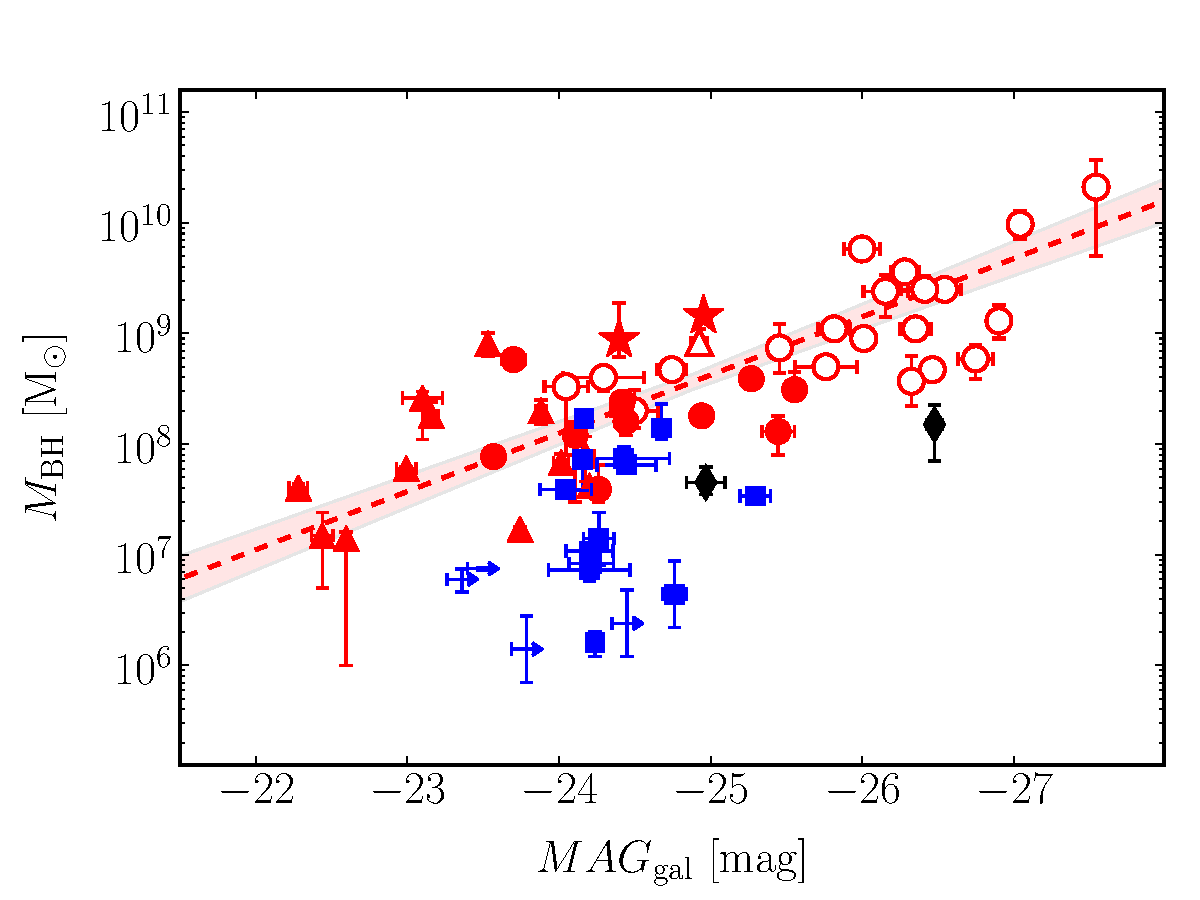
\includegraphics[width=\columnwidth]{images/mbh_vs_mag_tot.pdf}
\caption{Black hole mass plotted against $3.6\rm~\mu m$ galaxy absolute magnitude. 
Symbols are coded according to the galaxy morphological type: red circle = E, red star = E/S0, 
red upward triangle = S0, blue downward triangle = S0/Sp, blue square = Sp, black diamond = merger. 
Empty symbols represent core-S\'ersic spheroids, whereas filled symbols are used for S\'ersic spheroids. 
Four spiral galaxies had their magnitudes overestimated and are shown as upper limits. 
The red dashed line indicates the BCES bisector linear regression for the 45 early-type galaxies (E+S0), 
with the red shaded area denoting its $1\sigma$ uncertainty. 
We were not able to obtain any meaningful linear regression for the 13 ($=17-4$) late-type (Sp) galaxies. 
$M_{\rm BH}$ correlates equally well with $L_{\rm sph}$ and $L_{\rm gal}$ only for early-type galaxies, 
but not for all (early+late) galaxies. }
\label{fig:mbhmaggal}
\end{center}
\end{figure}

\begin{table*}
\centering
\caption{Linear regression analysis of the $M_{\rm BH} - L_{\rm gal}$ diagram.}
\begin{tabular}{llccccc}
\tableline\tableline
{\bf Subsample (size)} & {\bf Regression} & $\boldsymbol \alpha$ & $\boldsymbol \beta$ & $\boldsymbol \langle MAG_{\rm gal} \rangle$ & $\boldsymbol \epsilon$ & $\boldsymbol \Delta$ \\ 
\tableline 
\\
  & \multicolumn{6}{l}{$\log[M_{\rm BH}/{\rm M_\odot}] = \alpha + \beta[(MAG_{\rm gal} - \langle MAG_{\rm gal} \rangle)/{\rm mag}]$} \\ [0.5em]
 All (62)               & BCES $(Y|X)$   & $8.26 \pm 0.08$ & $-0.49 \pm 0.06$ & $-24.78$ & $-$ & $0.64$ \\
                        & BCES $(X|Y)$   & $8.26 \pm 0.12$ & $-1.01 \pm 0.15$ & $-24.78$ & $-$ & $0.92$ \\
                        & BCES Bisector  & $8.26 \pm 0.09$ & $-0.72 \pm 0.07$ & $-24.78$ & $-$ & $0.71$ \\
                        & mFITEXY $(Y|X)$  & $8.26^{+0.08}_{-0.08}$ & $-0.49^{+0.06}_{-0.07}$ & $-24.78$ & $0.61^{+0.07}_{-0.06}$ & $0.64$ \\
                        & mFITEXY $(X|Y)$  & $8.26^{+0.11}_{-0.12}$ & $-1.03^{+0.13}_{-0.16}$ & $-24.78$ & $0.88^{+0.10}_{-0.08}$ & $0.93$ \\
                        & mFITEXY Bisector & $8.26^{+0.10}_{-0.10}$ & $-0.73^{+0.09}_{-0.10}$ & $-24.78$ & $-$    & $0.71$ \\
                        & {\tt linmix\_err} $(Y|X)$  & $8.26 \pm 0.09$ & $-0.49 \pm 0.07$ & $-24.78$ & $0.63 \pm 0.07$ & $0.64$ \\
                        & {\tt linmix\_err} $(X|Y)$  & $8.26 \pm 0.12$ & $-1.02 \pm 0.15$ & $-24.78$ & $0.91 \pm 0.17$ & $0.93$ \\
                        & {\tt linmix\_err} Bisector & $8.26 \pm 0.10$ & $-0.72 \pm 0.15$ & $-24.78$ & $-$    & $0.71$ \\ [0.5em]

 Early-type (E+S0) (45) & BCES $(Y|X)$   & $8.56 \pm 0.07$ & $-0.44 \pm 0.05$ & $-24.88$ & $-$ & $0.45$ \\
                        & BCES $(X|Y)$   & $8.56 \pm 0.08$ & $-0.64 \pm 0.05$ & $-24.88$ & $-$ & $0.53$ \\
                        & BCES Bisector  & $8.56 \pm 0.07$ & $-0.53 \pm 0.04$ & $-24.88$ & $-$ & $0.47$ \\
                        & mFITEXY $(Y|X)$  & $8.56^{+0.06}_{-0.06}$ & $-0.42^{+0.05}_{-0.05}$ & $-24.88$ & $0.41^{+0.06}_{-0.05}$ & $0.45$ \\
                        & mFITEXY $(X|Y)$  & $8.56^{+0.08}_{-0.08}$ & $-0.66^{+0.07}_{-0.08}$ & $-24.88$ & $0.51^{+0.07}_{-0.06}$ & $0.55$ \\
                        & mFITEXY Bisector & $8.56^{+0.07}_{-0.07}$ & $-0.54^{+0.06}_{-0.06}$ & $-24.88$ & $-$    & $0.47$ \\
                        & {\tt linmix\_err} $(Y|X)$  & $8.56 \pm 0.07$ & $-0.42 \pm 0.06$ & $-24.88$ & $0.43 \pm 0.06$ & $0.45$ \\
                        & {\tt linmix\_err} $(X|Y)$  & $8.56 \pm 0.09$ & $-0.65 \pm 0.08$ & $-24.88$ & $0.53 \pm 0.10$ & $0.54$ \\
                        & {\tt linmix\_err} Bisector & $8.56 \pm 0.08$ & $-0.53 \pm 0.10$ & $-24.88$ & $-$    & $0.47$ \\

%Late-type (Sp) (13) & BCES $(Y|X)$      & $7.37 \pm 0.17$ & $-0.33 \pm 0.87$   & $-24.39$ & $-$ & $0.65$ \\
%                    & BCES $(X|Y)$      & $7.37 \pm 1.97$ & $-21.66 \pm 53.74$ & $-24.39$ & $-$ & $7.73$ \\
%                    & BCES Bisector     & $7.37 \pm 0.20$ & $-1.32 \pm 0.94$   & $-24.39$ & $-$ & $0.77$ \\
%                    & FITEXY $(Y|X)$    & $7.38^{+0.17}_{-0.18}$ & $-0.34^{+0.74}_{-0.80}$ & $-24.39$ & $0.63^{+0.19}_{-0.11}$ & $0.65$ \\
%                    & FITEXY $(X|Y)$    & $$ & $$ & $-24.39$ & $$ & $$ \\
%                    & FITEXY Bisector   & $$ & $$ & $-24.39$ & $-$    & $$ \\
%                    & {\tt linmix\_err} $(Y|X)$     & $$ & $$ & $-24.39$ & $$ & $$ \\
%                    & {\tt linmix\_err} $(X|Y)$     & $$ & $$ & $-24.39$ & $$ & $$ \\
%                    & {\tt linmix\_err} Bisector    & $$ & $$ & $-24.39$ & $-$    & $$ \\

%All (62)               & BCES $(Y|X)$   & $$ & $$ & $$ & $-$ & $$ \\
%                       & BCES $(X|Y)$   & $$ & $$ & $$ & $-$ & $$ \\
%                       & BCES Bisector     & $$ & $$ & $$ & $-$ & $$ \\
%                       & FITEXY $(Y|X)$ & $$ & $$ & $$ & $$ & $$ \\
%                       & FITEXY $(X|Y)$ & $$ & $$ & $$ & $$ & $$ \\
%                       & FITEXY Bisector   & $$ & $$ & $$ & $-$    & $$ \\
%                       & {\tt linmix\_err} $(Y|X)$  & $$ & $$ & $$ & $$ & $$ \\
%                       & {\tt linmix\_err} $(X|Y)$  & $$ & $$ & $$ & $$ & $$ \\
%                       & {\tt linmix\_err} Bisector    & $$ & $$ & $$ & $-$    & $$ \\

\tableline 
\tableline
\end{tabular}
\label{tab:lreggal} 
\tablecomments{For each subsample, we indicate $\langle MAG_{\rm gal} \rangle$, its average value of galaxy magnitudes. 
In the last two columns, we report $\epsilon$, the intrinsic scatter, and $\Delta$, the total rms scatter in the $\log(M_{\rm BH})$ direction. 
Four spiral galaxies had their luminosities underestimated and thus are not included in the linear regression analysis 
(the sample of all galaxies contains 66-4=62 objects). 
When considering all galaxies, irrespective of their morphological type, 
the $M_{\rm BH} - L_{\rm gal}$ correlation is weaker than the $M_{\rm BH} - L_{\rm sph}$ correlation, in terms of intrinsic scatter. 
However, when considering only early-type galaxies, the $M_{\rm BH} - L_{\rm gal}$ and $M_{\rm BH} - L_{\rm sph}$ correlations 
have consistent intrinsic scatter. }
\end{table*}

\subsection{Black hole mass -- spheroid luminosity}
The $M_{\rm BH} - L_{\rm sph}$ diagram is shown in Figure \ref{fig:mbhmagsph}, 
and the linear regression analysis is presented in Table \ref{tab:lregsph}. \\
S\'ersic and core-S\'ersic spheroids have slopes consistent with each other (within their $1\sigma$ uncertainties), 
in disagreement with the findings of GS13. 
The slope that we obtained for core-S\'ersic spheroids ($M_{\rm BH} \propto L_{\rm sph}^{1.18 \pm 0.20}$) 
is consistent with the slope reported by GS13 in the $K_s$-band for the same population ($M_{\rm BH} \propto L_{\rm sph}^{1.10 \pm 0.20}$). 
However, the slope that we determined for S\'ersic spheroids ($M_{\rm BH} \propto L_{\rm sph}^{1.53 \pm 0.20}$) 
is notably shallower than that found by GS13 ($M_{\rm BH} \propto L_{\rm sph}^{2.73 \pm 0.55}$). 
Although the S\'ersic/core-S\'ersic classification used by GS13 slightly differs\footnote{The classification has changed for the galaxies 
NGC 1316, NGC 1332 and NGC 3998.} from the classification used here, 
the main cause of such inconsistency is that the bulge-to-total ratios obtained from our galaxy decompositions 
are different from those assumed by GS13 to convert galaxy luminosities into bulge luminosities.
Our bulge-to-total ratios for low-luminosity S\'ersic spheroids ($3.6\rm~\mu m$ $MAG_{\rm sph} \gtrsim -22 \rm~mag$) 
are smaller than those used by GS13. 
The host galaxies of such bulges are late-type, spiral galaxies, 
which typically present a complex morphology (bars, double bars, embedded disks, nuclear components, etc).
Our sophisticated galaxy models account for the extra components, 
while the bulge-to-total ratios of GS13 were based on simple literature S\'ersic-bulge/exponential-disk decompositions 
which overestimated the bulge luminosity.
This results in our bulge magnitudes being on average $\sim$$1\rm~mag$ fainter than in GS13, after accounting for the different wavelength of the data.
At the same time, our bulge-to-total ratios for the high-luminosity S\'ersic spheroids ($3.6\rm~\mu m$ $MAG_{\rm sph} \lesssim -24 \rm~mag$) 
are on average larger than those adopted by GS13.
In this regime, the host systems are early-type galaxies that feature intermediate-scale disks\footnote{Intermediate-scale disks are 
disks of stars fully embedded in the spheroidal component of their galaxy. 
They are typical of ``disky'' elliptical galaxies (e.g.~NGC 3377), 
but they can also be found in other types of host galaxies.
They can be considered an intermediate class between nuclear disks, with sizes $\sim$$10-100\rm~pc$, %%
and large-scale disks, that encase the bulge and dominate the light at large radii.}. 
Past bulge/disk decompositions failed to correctly identify the extent of such disks and treated them as large-scale disks, 
thus underestimating the bulge luminosity.
The magnitudes that we obtained for such spheroids are on average $\sim$$1\rm~mag$ brighter than in GS13. 
These two effects explain the shallower slope that we obtained for the S\'ersic spheroids. \\
We have seen that the change in slope of the $M_{\rm BH} - L_{\rm sph}$ relation -- 
which is expected for consistency with other scaling relations 
(a single power-law $M_{\rm BH} - \sigma$ correlation and a double power-law $L_{\rm sph} - \sigma$ correlation) -- 
cannot be attributed to the division between the two populations of S\'ersic and core-S\'ersic spheroids.
We now test a new hypothesis, where the change in slope is ascribed to the different formation mechanisms of early- and late-type galaxies. 
If this hypothesis is correct, 
the spheroids of early-type galaxies will follow $M_{\rm BH} \propto L_{\rm sph}^{\sim 1}$, 
whereas the spheroids of late-type galaxies will have $M_{\rm BH} \propto L_{\rm sph}^{\sim 2.5}$.
First, we checked that elliptical and lenticular galaxies, taken separately, have slopes consistent with each other, 
and thus, taken together, they define a single \emph{red sequence} in the $M_{\rm BH} - L_{\rm sph}$ diagram. 
We then fit the bulges of early- and late-type galaxies with two separate log-linear regressions, 
and obtained $M_{\rm BH} \propto L_{\rm sph}^{1.00 \pm 0.10}$ and $M_{\rm BH} \propto L_{\rm sph}^{2.88 \pm 0.68}$ respectively, 
in excellent agreement with the theoretical expectations of our hypothesis. \\
%{\bf vertical scatter along the early type sequence is constant? if 2 overmassive bhs removed, what happens?}
We point out the unsuitability of Pearson's and Spearman's correlation coefficients because 
they do not take into account the error bars on our data.
Similarly, a visual inspection of the plotted data requires us to take into account the error bars 
when judging-by-eye the strength of a correlation. 
We have therefore relied on the quantitative regression analysis rather than subjective approaches.

\subsubsection{Pseudo- versus classical bulges}
Current views distinguish between classical bulges, which are considered to be spheroidal, pressure-supported systems, 
formed through violent processes, such as hierarchical clustering via minor mergers, 
and pseudo-bulges, thought to be disk-like, rotation-supported systems, 
built from secular evolution processes, such as instabilities of their surrounding disk or bar. 
Pseudo-bulges are notoriously hard to identify \citep{graham2013review,graham2014review,graham2015pseudo,graham2015review}.
For example, mergers can create bulges that rotate (e.g.~\citealt{bekki2010,keselmannusser2012}), 
and bars can spin-up classical bulges (e.g.~\citealt{saha2012}), 
thus rotation is not a definitive signature of a pseudo-bulge. 
Furthermore, many galaxies host both a pseudo- and a classical bulge (e.g.~\citealt{erwin2003,erwin2015,athanassoula2005,Gadotti2009,
macarthur2009,dosanjosdasilva2013,seidel2015}). 
In the recent literature, pseudo- and classical bulges have frequently been divided at the 
S\'ersic index $n_{\rm sph}=2$ (e.g.~\citealt{sani2011,beifiori2012}), 
although, from a selection of hundreds of disc galaxies imaged in the $K$-band, 
\cite{grahamworley2008} observed no bimodality in the bulge S\'ersic indices about $n_{\rm sph}=2$ or any other value. 
While pseudo-bulges are expected to have exponential-like surface brightness profiles ($n_{\rm sph} \simeq 1$), 
being disky components that formed from their surrounding exponential disks 
(e.g.~\citealt{bardeen1975,hohl1975,combessanders1981,combes1990,pfennigerfriedli1991}), 
it has been shown that mergers can create bulges with $n_{\rm sph}<2$
(e.g.~\citealt{elichemoral2011,scannapieco2011,querejeta2015}), 
just as low-luminosity elliptical galaxies (not built from the secular evolution of a disk)
are well known to have $n_{\rm sph}<2$ and even $n_{\rm sph}<1$ (e.g.~\citealt{davies1988,youngcurrie1994,jerjen2000}). 
The use of the S\'ersic index to identify pseudo-bulges is thus a dangerous practice. \\
\cite{sani2011} reported that pseudo-bulges -- which they labelled as such according to the $n_{\rm sph}<2$ criterion -- 
with low black hole masses ($M_{\rm BH} < 10^7\rm~M_\odot$) are significantly displaced from the correlation 
traced by their (classical) bulges with $n_{\rm sph}>2$. 
In Figure \ref{fig:pseudob}, we show the distribution of spheroid S\'ersic indices\footnote{The spheroid S\'ersic indices 
are taken from our galaxy decompositions (\emph{Paper I}).} 
in the $M_{\rm BH} - L_{\rm sph}$ diagram.
Our aim is to check whether bulges with $n_{\rm sph}<2$ 
are offset to lower black hole masses from the correlation defined by bulges with $n_{\rm sph}>2$. 
To do this, we fit a symmetrical linear regression to the bulges that have $n_{\rm sph}>2$ 
and we compute the vertical offset of all bulges from the regression. 
In Figure \ref{fig:pseudob}, we plot the vertical offset against $n_{\rm sph}$. 
Among the 23 bulges with $n_{\rm sph}<2$, 12 have a positive vertical offset and 11 have a negative vertical offset. 
\cite{kormendy2015review} provides a list of many pseudo-bulges classification criteria, including the divide at $n_{\rm sph}=2$, 
and cautions that each individual criterion has a failure rate of 0-25\%. 
If this is true, we should have that no less than 75\% of bulges with $n_{\rm sph}<2$ display a negative vertical offset\footnote{One 
reaches the same conclusion when using the vertical offset from the correlation defined by bulges with $n_{\rm sph}>3$ or even $n_{\rm sph}>4$. 
There are 13 and 10 bulges with $n_{\rm sph}<2$ that lie above and below, respectively, the correlation traced by bulges with $n_{\rm sph}>3$. 
Similarly, there are 15 and 8 bulges with $n_{\rm sph}<2$ that lie above and below, respectively, the correlation traced by bulges with $n_{\rm sph}>4$.}. 
What we observe, instead, is that there are the same number of bulges with $n_{\rm sph}<2$ lying above and below 
the correlation defined by bulges with $n_{\rm sph}>2$, 
and that the amplitude of their offset is the same ($\lesssim 1.5\rm~dex$).
That is, bulges with $n_{\rm sph}<2$ do not appear to be offset from the correlation traced by bulges with $n_{\rm sph}>2$. 


\begin{figure}[h]
\begin{center}
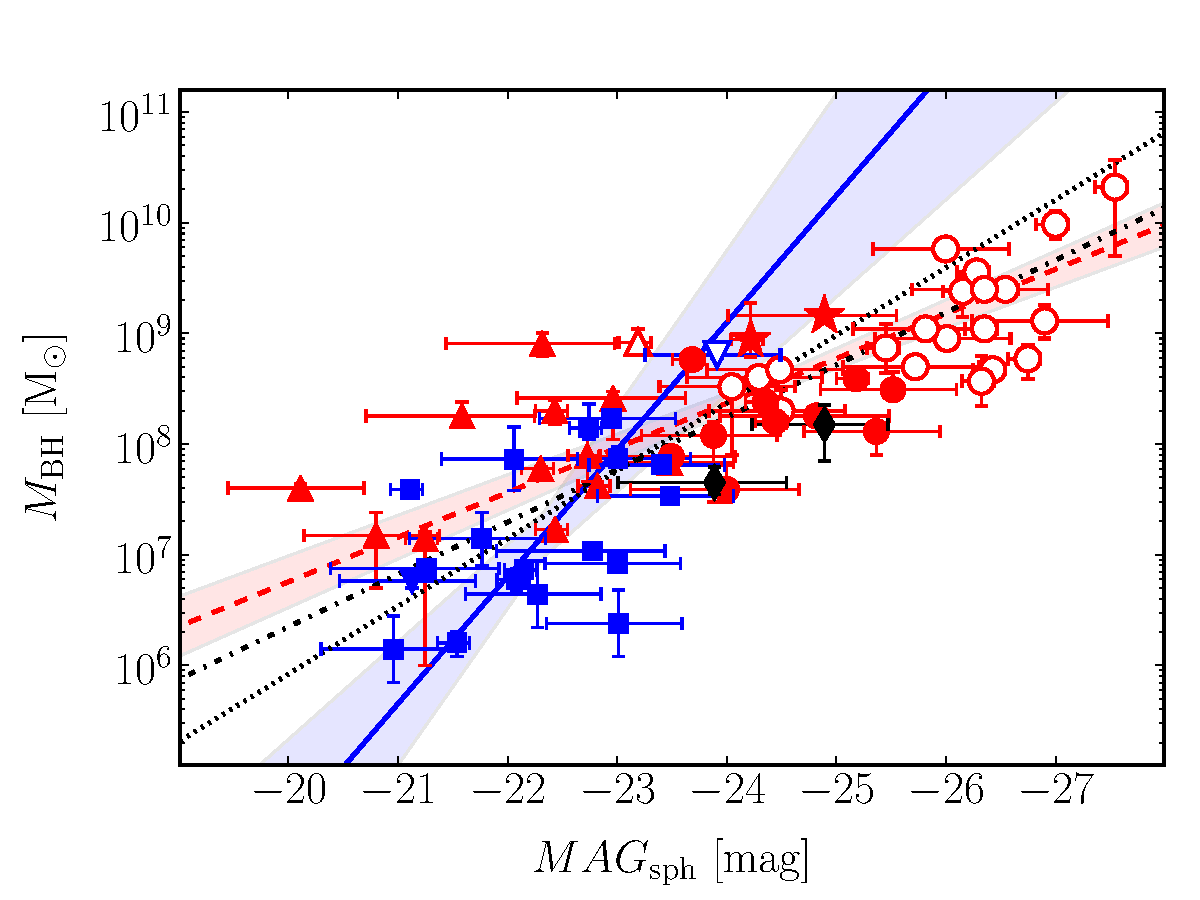
\includegraphics[width=\columnwidth]{images/mbh_vs_mag_sph.pdf}
\caption{Black hole mass plotted against $3.6\rm~\mu m$ spheroid absolute magnitude. 
Symbols are coded according to the galaxy morphological type: red circle = E, red star = E/S0, 
red upward triangle = S0, blue downward triangle = S0/Sp, blue square = Sp, black diamond = merger. 
Empty symbols represent core-S\'ersic spheroids, whereas filled symbols are used for S\'ersic spheroids. 
The red dashed line indicates the BCES bisector linear regression for the bulges of the 45 early-type (E+S0) galaxies, 
with the red shaded area denoting its $1\sigma$ uncertainty. 
The blue solid line shows the BCES bisector linear regression for the bulges of the 17 late-type (Sp) galaxies, 
with the blue shaded area denoting its $1\sigma$ uncertainty. 
The black dashed-dotted and dotted lines represent the BCES bisector linear regressions for the core-S\'ersic and S\'ersic spheroids, respectively.}
\label{fig:mbhmagsph}
\end{center}
\end{figure}

\begin{figure}[h]
\begin{center}
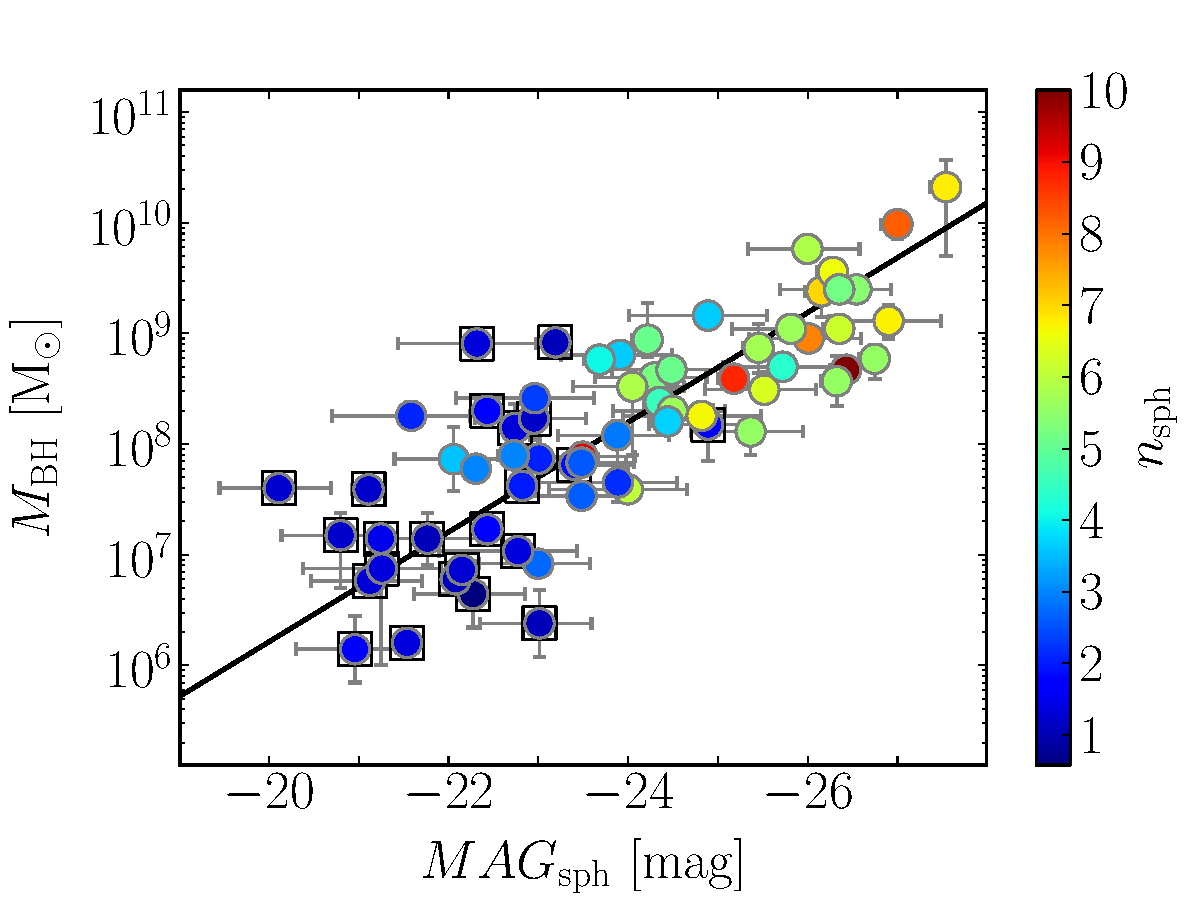
\includegraphics[width=\columnwidth]{images/mbh_vs_mag_sph_psb.pdf}
\caption{Black hole mass plotted against $3.6\rm~\mu m$ spheroid absolute magnitude. 
Symbols are color coded according to the spheroid S\'ersic index $n_{\rm sph}$. 
Bulges with $n_{\rm sph}<2$, claimed by some to be pseudo-bulges, are marked with a square. 
The black solid line shows the BCES bisector linear regression for the spheroids that have $n_{\rm sph} \geq 2$, 
such that $M_{\rm BH} \propto L_{\rm sph}^{1.25 \pm 0.13}$. }
\label{fig:pseudob}
\end{center}
\end{figure}


\begin{figure}[h]
\begin{center}
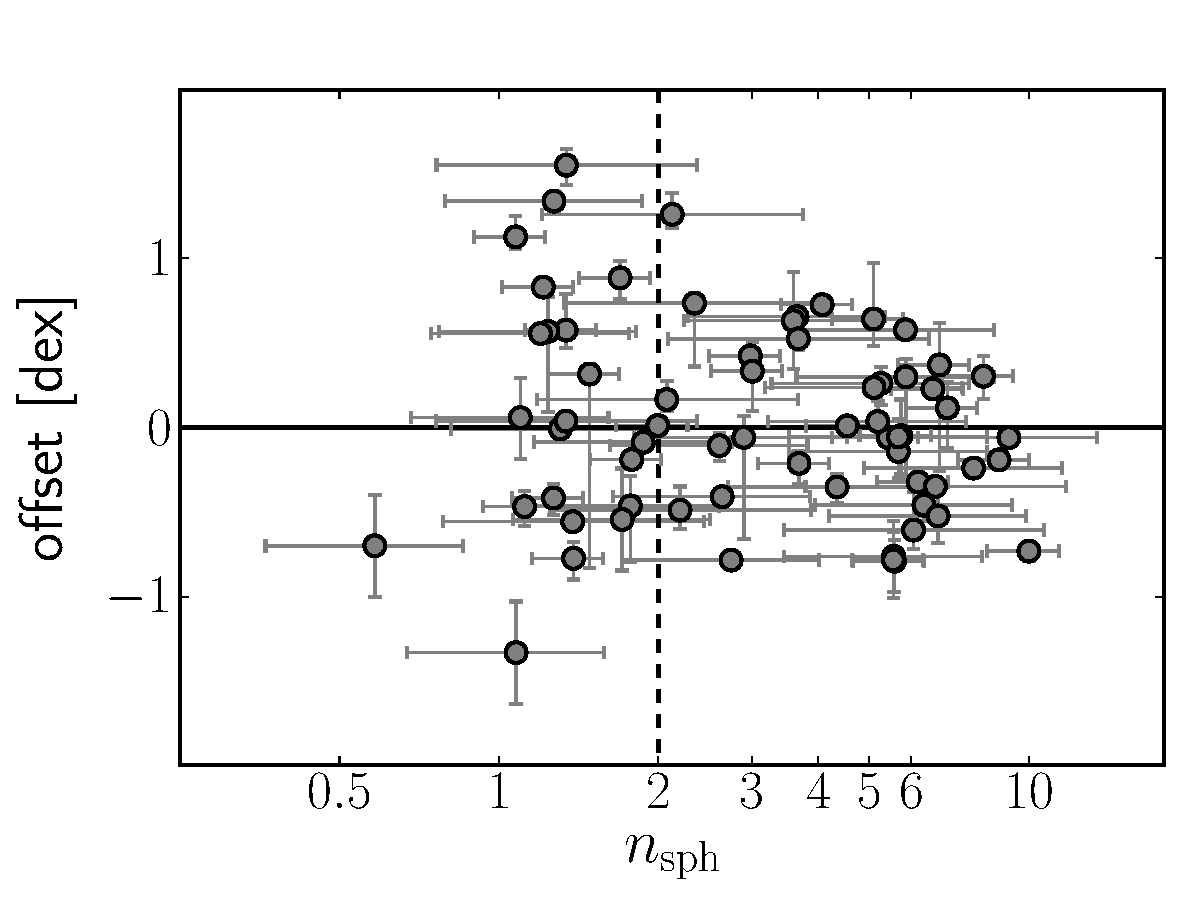
\includegraphics[width=\columnwidth]{images/inset_psb.pdf}
\caption{Vertical offset from the $M_{\rm BH} - L_{\rm sph}$ correlation defined by spheroids with $n_{\rm sph} \geq 2$ (see Figure \ref{fig:pseudob}), 
plotted against $n_{\rm sph}$. 
The vertical dashed line corresponds to $n_{\rm sph} = 2$.
The horizontal solid line is equivalent to a zero vertical offset.
Among the bulges with $n_{\rm sph}<2$, 12 have a positive vertical offset and 11 have a negative vertical offset.
Hence, bulges with $n_{\rm sph}<2$ are not randomly offset to lower black hole masses 
from the correlation traced by bulges with $n_{\rm sph} \geq 2$.}
\label{fig:offset}
\end{center}
\end{figure}


\begin{table*}
\centering
\caption{Linear regression analysis of the $M_{\rm BH} - L_{\rm sph}$ diagram.}
\begin{tabular}{llccccc}
\tableline
\tableline
{\bf Subsample (size)} & {\bf Regression} & $\boldsymbol \alpha$ & $\boldsymbol \beta$ & $\boldsymbol \langle MAG_{\rm sph} \rangle$ & $\boldsymbol \epsilon$ & $\boldsymbol \Delta$ \\ 
\tableline 
\\
 & \multicolumn{6}{l}{$\log[M_{\rm BH}/{\rm M_\odot}] = \alpha + \beta[(MAG_{\rm sph} - \langle MAG_{\rm sph} \rangle)/{\rm mag}]$} \\ [0.5em]
All (66)               & BCES $(Y|X)$   & $8.16 \pm 0.07$ & $-0.44 \pm 0.04$ & $-23.86$ & $-$ & $0.56$ \\
                       & BCES $(X|Y)$   & $8.16 \pm 0.08$ & $-0.61 \pm 0.05$ & $-23.86$ & $-$ & $0.68$ \\
                       & BCES Bisector  & $8.16 \pm 0.07$ & $-0.52 \pm 0.04$ & $-23.86$ & $-$ & $0.60$ \\
                       & mFITEXY $(Y|X)$    & $8.17^{+0.06}_{-0.07}$ & $-0.43^{+0.03}_{-0.04}$ & $-23.86$ & $0.49^{+0.06}_{-0.05}$ & $0.56$ \\
                       & mFITEXY $(X|Y)$    & $8.15^{+0.07}_{-0.08}$ & $-0.61^{+0.05}_{-0.05}$ & $-23.86$ & $0.58^{+0.07}_{-0.06}$ & $0.68$ \\
                       & mFITEXY Bisector   & $8.16^{+0.07}_{-0.07}$ & $-0.51^{+0.04}_{-0.04}$ & $-23.86$ & $-$    & $0.60$ \\
                       & {\tt linmix\_err} $(Y|X)$     & $8.16 \pm 0.07$ & $-0.42 \pm 0.04$ & $-23.86$ & $0.51 \pm 0.06$ & $0.56$ \\
                       & {\tt linmix\_err} $(X|Y)$     & $8.16 \pm 0.09$ & $-0.60 \pm 0.06$ & $-23.86$ & $0.60 \pm 0.09$ & $0.67$ \\
                       & {\tt linmix\_err} Bisector    & $8.16 \pm 0.08$ & $-0.51 \pm 0.09$ & $-23.86$ & $-$    & $0.59$ \\ [0.5em]

$n>2$ (43)             & BCES $(Y|X)$      & $8.58 \pm 0.07$ & $-0.42 \pm 0.06$ & $-24.77$ & $-$ & $0.46$ \\
                       & BCES $(X|Y)$      & $8.58 \pm 0.08$ & $-0.58 \pm 0.06$ & $-24.77$ & $-$ & $0.56$ \\
                       & BCES Bisector     & $8.58 \pm 0.07$ & $-0.50 \pm 0.05$ & $-24.77$ & $-$ & $0.49$ \\
                       & mFITEXY $(Y|X)$    & $8.57^{+0.07}_{-0.06}$ & $-0.41^{+0.04}_{-0.04}$ & $-24.77$ & $0.38^{+0.06}_{-0.06}$ & $0.46$ \\
                       & mFITEXY $(X|Y)$    & $8.56^{+0.08}_{-0.08}$ & $-0.57^{+0.06}_{-0.07}$ & $-24.77$ & $0.44^{+0.08}_{-0.11}$ & $0.55$ \\
                       & mFITEXY Bisector   & $8.57^{+0.07}_{-0.07}$ & $-0.49^{+0.05}_{-0.05}$ & $-24.77$ & $-$    & $0.49$ \\
                       & {\tt linmix\_err} $(Y|X)$     & $8.56 \pm 0.07$ & $-0.39 \pm 0.05$ & $-24.77$ & $0.40 \pm 0.06$ & $0.46$ \\
                       & {\tt linmix\_err} $(X|Y)$     & $8.55 \pm 0.09$ & $-0.57 \pm 0.08$ & $-24.77$ & $0.49 \pm 0.10$ & $0.55$ \\
                       & {\tt linmix\_err} Bisector    & $8.56 \pm 0.08$ & $-0.48 \pm 0.10$ & $-24.77$ & $-$    & $0.49$ \\  [0.5em]
                   
Core-S\'ersic (22) & BCES $(Y|X)$   & $9.06 \pm 0.09$ & $-0.32 \pm 0.11$  & $-25.73$ & $-$    & $0.42$ \\
                   & BCES $(X|Y)$   & $9.06 \pm 0.12$ & $-0.65 \pm 0.12$  & $-25.73$ & $-$    & $0.61$ \\
                   & BCES Bisector  & $9.06 \pm 0.10$ & $-0.47 \pm 0.08$  & $-25.73$ & $-$    & $0.48$ \\
                   & mFITEXY $(Y|X)$   & $9.06^{+0.08}_{-0.09}$ & $-0.26^{+0.08}_{-0.07}$ & $-25.73$ & $0.36^{+0.09}_{-0.06}$ & $0.42$ \\
                   & mFITEXY $(X|Y)$   & $9.03^{+0.15}_{-0.16}$ & $-0.72^{+0.17}_{-0.31}$ & $-25.73$ & $0.61^{+0.14}_{-0.09}$ & $0.68$ \\
                   & mFITEXY Bisector  & $9.05^{+0.12}_{-0.13}$ & $-0.47^{+0.12}_{-0.17}$ & $-25.73$ & $-$    & $0.48$ \\
                   & {\tt linmix\_err} $(Y|X)$  & $9.04 \pm 0.10$ & $-0.24 \pm 0.09$ & $-25.73$ & $0.40 \pm 0.08$ & $0.42$ \\
                   & {\tt linmix\_err} $(X|Y)$  & $9.03 \pm 0.17$ & $-0.69 \pm 0.27$ & $-25.73$ & $0.68 \pm 0.30$ & $0.64$ \\
                   & {\tt linmix\_err} Bisector & $9.04 \pm 0.14$ & $-0.44 \pm 0.16$ & $-25.73$ & $-$    & $0.46$ \\ [0.5em]

S\'ersic (44) & BCES $(Y|X)$   & $7.71 \pm 0.09$ & $-0.41 \pm 0.08$ & $-22.92$ & $-$    & $0.61$ \\
              & BCES $(X|Y)$   & $7.71 \pm 0.14$ & $-0.86 \pm 0.16$ & $-22.92$ & $-$    & $0.93$ \\
              & BCES Bisector  & $7.71 \pm 0.10$  & $-0.61 \pm 0.08$ & $-22.92$ & $-$    & $0.71$ \\
              & mFITEXY $(Y|X)$   & $7.72^{+0.08}_{-0.09}$ & $-0.41^{+0.07}_{-0.08}$ & $-22.92$ & $0.54^{+0.08}_{-0.07}$ & $0.61$ \\
              & mFITEXY $(X|Y)$   & $7.72^{+0.14}_{-0.13}$ & $-0.86^{+0.13}_{-0.19}$ & $-22.92$ & $0.77^{+0.13}_{-0.10}$ & $0.93$ \\
              & mFITEXY Bisector  & $7.72^{+0.11}_{-0.11}$ & $-0.61^{+0.10}_{-0.12}$ & $-22.92$ & $-$                    & $0.71$ \\
              & {\tt linmix\_err} $(Y|X)$  & $7.73 \pm 0.09$ & $-0.41 \pm 0.08$ & $-22.92$ & $0.55 \pm 0.08$ & $0.61$ \\
              & {\tt linmix\_err} $(X|Y)$  & $7.73 \pm 0.14$ & $-0.86 \pm 0.17$ & $-22.92$ & $0.79 \pm  0.20$ & $0.93$ \\
              & {\tt linmix\_err} Bisector & $7.73 \pm 0.12$ & $-0.62 \pm 0.15$ & $-22.92$ & $-$    & $0.71$ \\ [0.5em]

%Ellipticals (E) (30)   & BCES $(Y|X)$   & $8.80 \pm 0.07$ & $-0.53 \pm 0.09$ & $-25.45$ & $-$    & $0.42$ \\
%                      & BCES $(X|Y)$   & $8.80 \pm 0.08$ & $-0.66 \pm 0.07$ & $-25.45$ & $-$    & $0.48$ \\
%                      & BCES Bisector     & $8.80 \pm 0.08$ & $-0.59 \pm 0.07$ & $-25.45$ & $-$    & $0.44$ \\
%                      & FITEXY $(Y|X)$ & $8.81^{+0.07}_{-0.07}$ & $-0.44^{+0.06}_{-0.07}$ & $-25.45$ & $0.33$     & $0.40$ \\
%                      & FITEXY $(X|Y)$ & $8.78^{+0.09}_{-0.09}$ & $-0.7^{+0.1}_{-0.1}$    & $-25.45$ & $0.60$     & $0.50$\\
%                      & FITEXY Bisector   & $8.80^{+0.08}_{-0.08}$ & $-0.56^{+0.08}_{-0.10}$ & $-25.45$ & $-$        & $0.43$ \\
%
%Lenticulars (S0) (13)  & BCES $(Y|X)$   & $7.9 \pm 0.1$ & $-0.4 \pm 0.2$ & $-22.19$ & $-$    & $0.56$ \\
%                      & BCES $(X|Y)$   & $7.9 \pm 0.3$ & $-1.1 \pm 0.5$ & $-22.19$ & $-$    & $1.01$ \\
%                      & BCES Bisector     & $7.9 \pm 0.2$ & $-0.7 \pm 0.2$ & $-22.19$ & $-$    & $0.69$ \\
%                      & FITEXY $(Y|X)$ & $7.9^{+0.2}_{-0.1}$ & $-0.3^{+0.2}_{-0.2}$ & $-22.19$ & $0.51$     & $0.56$ \\
%                      & FITEXY $(X|Y)$ & $7.8^{+0.3}_{-0.4}$ & $-1.3^{+0.4}_{-1.3}$ & $-22.19$ & $0.71$     & $1.20$\\
%                      & FITEXY Bisector   & $7.9^{+0.2}_{-0.3}$ & $-0.7^{+0.3}_{-0.4}$ & $-22.19$ & $-$        & $0.71$ \\
%

{\bf Early-type (E+S0)} (45) & BCES $(Y|X)$    & $8.56 \pm 0.07$ & $-0.33 \pm 0.04$ & $-24.47$ & $-$    & $0.46$ \\
                             & BCES $(X|Y)$    & $8.56 \pm 0.08$ & $-0.48 \pm 0.05$ & $-24.47$ & $-$    & $0.55$ \\
                             & {\bf BCES Bisector}& $\boldsymbol{8.56 \pm 0.07}$ & $\boldsymbol{-0.40 \pm 0.04}$ & $\boldsymbol{-24.47}$ & $-$    & $\boldsymbol{0.49}$ \\
                             & mFITEXY $(Y|X)$ & $8.56^{+0.06}_{-0.06}$ & $-0.32^{+0.03}_{-0.04}$ & $-24.47$ & $0.40^{+0.06}_{-0.05}$ & $0.46$ \\
                             & mFITEXY $(X|Y)$ & $8.54^{+0.08}_{-0.08}$ & $-0.49^{+0.05}_{-0.06}$ & $-24.47$ & $0.49^{+0.08}_{-0.06}$ & $0.57$\\
                             & mFITEXY Bisector   & $8.55^{+0.07}_{-0.07}$ & $-0.41^{+0.04}_{-0.05}$ & $-24.47$ & $-$    & $0.49$ \\
                             & {\tt linmix\_err} $(Y|X)$  & $8.55 \pm 0.07$ & $-0.32 \pm 0.04$ & $-24.47$ & $0.41 \pm 0.06$ & $0.46$ \\
                             & {\tt linmix\_err} $(X|Y)$  & $8.55 \pm 0.09$ & $-0.48 \pm 0.06$ & $-24.47$ & $0.51 \pm 0.10$ & $0.56$ \\
                             & {\tt linmix\_err} Bisector    & $8.55 \pm 0.08$ & $-0.40 \pm 0.09$ & $-24.47$ & $-$    & $0.49$ \\ [0.5em]

{\bf Late-type (Sp)} (17) & BCES $(Y|X)$    & $7.18 \pm 0.16$ & $-0.79 \pm 0.43$ & $-22.33$ & $-$    & $0.70$ \\
                          & BCES $(X|Y)$    & $7.18 \pm 0.29$ & $-1.71 \pm 0.71$ & $-22.33$ & $-$    & $1.26$ \\
                          & {\bf BCES Bisector}& $\boldsymbol{7.18 \pm 0.20}$ & $\boldsymbol{-1.15 \pm 0.27}$ & $\boldsymbol{-22.33}$ & $-$    & $\boldsymbol{0.88}$ \\
                          & mFITEXY $(Y|X)$    & $7.20^{+0.15}_{-0.15}$ & $-0.53^{+0.22}_{-0.24}$ & $-22.33$ & $0.55^{+0.15}_{-0.10}$ & $0.63$ \\
                          & mFITEXY $(X|Y)$    & $7.38^{+0.54}_{-0.36}$ & $-2.02^{+0.71}_{-2.13}$ & $-22.33$ & $1.09^{+0.41}_{-0.24}$ & $1.50$ \\
                          & mFITEXY Bisector   & $7.26^{+0.40}_{-0.28}$ & $-1.03^{+0.33}_{-0.52}$ & $-22.33$ & $-$    & $0.82$ \\
                          & {\tt linmix\_err} $(Y|X)$  & $7.24 \pm 0.19$ & $-0.46 \pm 0.32$ & $-22.33$ & $0.63 \pm 0.16$ & $0.62$ \\
                          & {\tt linmix\_err} $(X|Y)$  & $7.34 \pm 0.43$ & $-1.93 \pm 1.30$ & $-22.33$ & $1.31 \pm 0.97$ & $1.43$ \\
                          & {\tt linmix\_err} Bisector & $7.27 \pm 0.33$ & $-0.96 \pm 0.50$ & $-22.33$ & $-$    & $0.78$ \\

\tableline 
\tableline
\end{tabular}
\label{tab:lregsph} 
\tablecomments{For each subsample, we indicate $\langle MAG_{\rm sph} \rangle$, its average value of spheroid magnitudes. 
In the last two columns, we report $\epsilon$, the intrinsic scatter, and $\Delta$, the total rms scatter in the $\log(M_{\rm BH})$ direction. 
Both the early- and late-type subsamples do not contain the two galaxies classified as S0/Sp and the two galaxies classified as mergers (45+17=66-2-2). }
\end{table*}


\subsection{Black hole mass -- spheroid stellar mass}
Finally, we present the $M_{\rm BH} - M_{\rm *,sph}$ diagram in Figure \ref{fig:mbhmasssph}, 
and its linear regression analysis in Table \ref{tab:lregmass}. 
The bulges of early-type galaxies follow $M_{\rm BH} \propto M_{\rm *,sph}^{1.04 \pm 0.10}$,
consistent with a dry-merging formation scenario,
and define a tight \emph{red sequence} with intrinsic scatter $\epsilon_{(Y|X)} = 0.43 \pm 0.06\rm~dex$. 
On the other hand, the bulges of spiral galaxies trace a steeper \emph{blue sequence}, 
whose slope is less well constrained due to the small size of the subsample and, more importantly, 
to the small range in $M_{\rm *,sph}$ that the subsample spans. 
More data would be welcome to better constrain the slope of this \emph{blue sequence}.
For the bulges of spiral galaxies, the BCES code returns a log-linear relation with slope $= 3.00 \pm 1.30$, 
while the modified FITEXY routine finds a shallower (but still consistent within the $1\sigma$ uncertainty) 
slope $= 2.28^{+1.67}_{-1.01}$.
The Bayesian estimator of \cite{linmixerr} fails in performing an inverse $(X|Y)$ linear regression for the subsample of spiral galaxies. 

Using data from \cite{jiang2011a}, 
\cite{grahamscott2015} collected a sample of $\sim$140 low-redshift ($z \leq 0.35$, with a median redshift $\langle z \rangle = 0.085$) 
bulges hosting Active Galactic Nuclei (AGNs) with 
black hole masses $10^5 \lesssim M_{\rm BH}/{\rm M_\odot} \lesssim 2 \times 10^6$, 
and showed that they roughly follow the quadratic $M_{\rm BH} - M_{\rm *,sph}$ relation defined by S\'ersic bulges. 
%Although we demonstrated that, using our dataset, the S\'ersic bulges do not define a quadratic relation, 
We anticipate here that the correlation traced by our bulges of spiral galaxies 
may track the location of the AGNs in the $M_{\rm BH} - M_{\rm *,sph}$ diagram.
That is, the AGNs appear to be the low-mass continuation of the tentative \emph{blue sequence} shown in Figure \ref{fig:mbhmasssph}. 
We additionally note that the majority of our spiral galaxies host an AGN\footnote{According to the nuclear classification reported on NED 
(Nasa Extragalactic Database), among our 17 spiral galaxies, at least 12 host a Seyfert AGN and one hosts a LINER AGN.}.
This topic will be investigated in Graham et al. (2015, \emph{in preparation}) with a dedicated analysis. \\
 

\begin{figure}[h]
\begin{center}
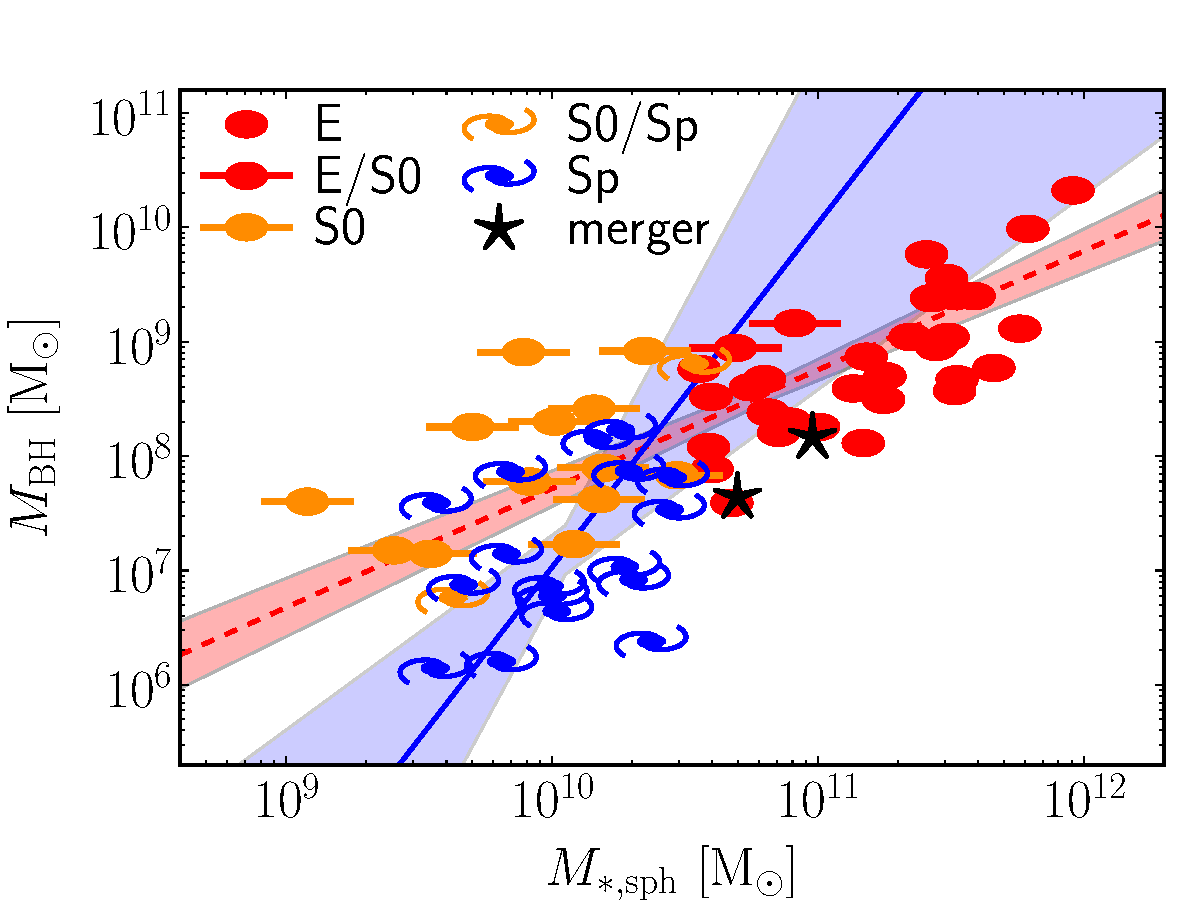
\includegraphics[width=\columnwidth]{images/mbh_vs_mass_sph.pdf}
\caption{Black hole mass plotted against spheroid stellar mass. 
Symbols are coded according to the galaxy morphological type.
The red dashed line indicates the BCES bisector linear regression for the bulges of the 45 early-type galaxies (E+S0), 
with the red shaded area denoting its $1\sigma$ uncertainty. 
The bulges of early-type galaxies follow $M_{\rm BH} \propto M_{\rm *,sph}^{1.04 \pm 0.10}$,
a near-linear relation consistent with a dry-merging formation scenario.
The steeper blue solid line shows the BCES bisector linear regression for the bulges of the 17 late-type (Sp) galaxies, 
with the blue shaded area denoting its $1\sigma$ uncertainty. 
The bulges of late-type galaxies follow $M_{\rm BH} \propto M_{\rm *,sph}^{2-3}$, 
indicating that gas-rich processes feed the black hole more efficiently (``quadratically'' or ``cubically'') than the host bulge grows in stellar mass. 
We note that AGNs with $10^5 \lesssim M_{\rm BH}/{\rm M_\odot} \lesssim 2 \times 10^6$ \citep{jiang2011a} appear to follow the blue line 
(see Graham et al. 2015, \emph{in preparation}).}
\label{fig:mbhmasssph}
\end{center}
\end{figure}

\begin{table*}
\centering
\caption{Linear regression analysis of the $M_{\rm BH} - M_{\rm *,sph}$ diagram.}
\begin{tabular}{llccccc}
\tableline
\tableline
{\bf Subsample (size)} & {\bf Regression} & $\boldsymbol \alpha$ & $\boldsymbol \beta$ & $\boldsymbol \langle M_{\rm *,sph} \rangle$ & $\boldsymbol \epsilon$ & $\boldsymbol \Delta$ \\ 
\tableline 
\\
  & \multicolumn{6}{l}{$\log[M_{\rm BH}/{\rm M_\odot}] = \alpha + \beta \log[(M_{\rm *,sph} - \langle M_{\rm *,sph} \rangle)/{\rm M_\odot}]$} \\ [0.5em]
 Core-S\'ersic (22)     & BCES $(Y|X)$      & $9.06 \pm 0.09$ & $0.86 \pm 0.28$ & $11.28$ & $-$ & $0.42$ \\
 			& BCES $(X|Y)$      & $9.06 \pm 0.12$ & $1.70 \pm 0.32$ & $11.28$ & $-$ & $0.61$ \\
 			& BCES Bisector     & $9.06 \pm 0.10$ & $1.19 \pm 0.23$ & $11.28$ & $-$ & $0.47$ \\
 			& FITEXY $(Y|X)$    & $9.06^{+0.08}_{-0.08}$ & $0.68^{+0.21}_{-0.20}$ & $11.28$ & $0.36^{+0.09}_{-0.06}$ & $0.42$ \\
 			& FITEXY $(X|Y)$    & $9.03^{+0.15}_{-0.16}$ & $1.90^{+0.85}_{-0.46}$ & $11.28$ & $0.62^{+0.13}_{-0.10}$ & $0.68$ \\
 			& FITEXY Bisector   & $9.05^{+0.12}_{-0.13}$ & $1.12^{+0.35}_{-0.27}$ & $11.28$ & $-$                    & $0.46$ \\
 			& {\tt linmix\_err} $(Y|X)$     & $9.04 \pm 0.10$ & $0.64 \pm 0.25$ & $11.28$ & $0.40 \pm 0.09$ & $0.42$ \\
 			& {\tt linmix\_err} $(X|Y)$     & $9.03 \pm 0.17$ & $1.80 \pm 0.70$ & $11.28$ & $0.67 \pm 0.30$ & $0.65$ \\
 			& {\tt linmix\_err} Bisector	& $9.04 \pm 0.14$ & $1.06 \pm 0.35$ & $11.28$ & $-$	& $0.45$ \\

 S\'ersic (44)		& BCES $(Y|X)$      & $7.71 \pm 0.09$ & $0.95 \pm 0.21$ & $10.25$ & $-$ & $0.64$ \\
 			& BCES $(X|Y)$      & $7.71 \pm 0.16$ & $2.52 \pm 0.54$ & $10.25$ & $-$ & $1.11$ \\
 			& BCES Bisector     & $7.71 \pm 0.11$ & $1.48 \pm 0.20$ & $10.25$ & $-$ & $0.74$ \\
 			& FITEXY $(Y|X)$    & $7.72^{+0.10}_{-0.09}$ & $0.96^{+0.21}_{-0.21}$ & $10.25$ & $0.58^{+0.09}_{-0.07}$ & $0.64$ \\
 			& FITEXY $(X|Y)$    & $7.72^{+0.16}_{-0.16}$ & $2.49^{+0.69}_{-0.45}$ & $10.25$ & $0.93^{+0.15}_{-0.13}$ & $1.10$ \\
 			& FITEXY Bisector   & $7.72^{+0.13}_{-0.13}$ & $1.49^{+0.33}_{-0.28}$ & $10.25$ & $-$    & $0.74$ \\
 			& {\tt linmix\_err} $(Y|X)$     & $7.73 \pm 0.10$ & $0.98 \pm 0.24$ & $10.25$ & $0.59 \pm 0.08$ & $0.65$ \\
 			& {\tt linmix\_err} $(X|Y)$     & $7.73 \pm 0.17$ & $2.48 \pm 0.59$ & $10.25$ & $0.95 \pm 0.27$ & $1.10$ \\
 			& {\tt linmix\_err} Bisector	& $7.73 \pm 0.14$ & $1.49 \pm 0.57$ & $10.25$ & $-$	& $0.74$ \\

{\bf Early-type (E+S0)} (45)  & BCES $(Y|X)$       & $8.56 \pm 0.07$ & $0.85 \pm 0.12$ & $10.81$ & $-$ & $0.48$ \\
                              & BCES $(X|Y)$       & $8.56 \pm 0.09$ & $1.27 \pm 0.13$ & $10.81$ & $-$ & $0.59$ \\
                              & {\bf BCES Bisector}& $\boldsymbol{8.56 \pm 0.07}$ & $\boldsymbol{1.04 \pm 0.10}$ & $\boldsymbol{10.81}$ & $-$ & $\boldsymbol{0.51}$ \\
                              & mFITEXY $(Y|X)$     & $8.56^{+0.06}_{-0.07}$ & $0.83^{+0.11}_{-0.11}$ & $10.81$ & $0.42^{+0.07}_{-0.05}$ & $0.48$ \\
                              & mFITEXY $(X|Y)$     & $8.54^{+0.08}_{-0.09}$ & $1.32^{+0.18}_{-0.15}$ & $10.81$ & $0.53^{+0.08}_{-0.07}$ & $0.61$ \\
                              & mFITEXY Bisector    & $8.55^{+0.07}_{-0.08}$ & $1.05^{+0.14}_{-0.12}$ & $10.81$ & $-$                    & $0.51$ \\
                              & {\tt linmix\_err} $(Y|X)$     & $8.55 \pm 0.07$ & $0.82 \pm 0.12$ & $10.81$ & $0.43 \pm 0.06$ & $0.48$ \\
                              & {\tt linmix\_err} $(X|Y)$     & $8.55 \pm 0.09$ & $1.29 \pm 0.17$ & $10.81$ & $0.54 \pm 0.11$ & $0.59$ \\
                              & {\tt linmix\_err} Bisector    & $8.55 \pm 0.08$ & $1.03 \pm 0.19$ & $10.81$ & $-$    & $0.51$ \\ [0.5em]

{\bf Late-type (Sp)} (17)    & BCES $(Y|X)$    & $7.18 \pm 0.17$ & $1.95 \pm 1.52$ & $10.05$ & $-$ & $0.74$ \\ 
                             & BCES $(X|Y)$    & $7.18 \pm 0.39$ & $5.89 \pm 3.40$ & $10.05$ & $-$ & $1.70$ \\
                             & {\bf BCES Bisector}& $\boldsymbol{7.18 \pm 0.21}$ & $\boldsymbol{3.00 \pm 1.30}$ & $\boldsymbol{10.05}$ & $-$ & $\boldsymbol{0.94}$ \\
                             & mFITEXY $(Y|X)$     & $7.20^{+0.15}_{-0.16}$ & $1.22^{+0.70}_{-0.62}$  & $10.05$ & $0.59^{+0.16}_{-0.11}$ & $0.66$ \\
                             & mFITEXY $(X|Y)$     & $7.44^{+1.45}_{-0.52}$ & $7.14^{+26.31}_{-3.01}$ & $10.05$ & $1.49^{+0.56}_{-0.36}$ & $2.08$ \\
                             & {\bf mFITEXY Bisector}    & $\boldsymbol{7.24^{+1.04}_{-0.39}}$ & $\boldsymbol{2.28^{+1.67}_{-1.01}}$  & $\boldsymbol{10.05}$ & $-$    & $\boldsymbol{0.79}$ \\
                             & {\tt linmix\_err} $(Y|X)$  & $7.23 \pm 0.19$ & $0.96 \pm 0.96$ & $10.05$ & $0.67 \pm 0.16$ & $0.65$ \\
                             & {\tt linmix\_err} $(X|Y)$  & $7.42 \pm 0.64$ & $6.96 \pm 6.73$ & $10.05$ & $1.83 \pm 1.86$ & $2.03$ \\
                             & {\tt linmix\_err} Bisector & $7.26 \pm 0.47$ & $1.94 \pm 216.38$ & $10.05$ & $-$    & $0.74$ \\
                  
\tableline 
\tableline
\end{tabular}
\label{tab:lregmass} 
\tablecomments{For each subsample, we indicate $\langle M_{\rm *,sph} \rangle$, its average value of spheroid stellar masses. 
In the last two columns, we report $\epsilon$, the intrinsic scatter, and $\Delta$, the total rms scatter in the $\log(M_{\rm BH})$ direction. }
\end{table*}

 

\section{Conclusions}
\label{sec:concl}
% %ngc0524 outlier, n1332 non outlier
% to be re-written
%
% \begin{itemize}
% \item The bulges of early-type (E + S0) galaxies follow $M_{\rm BH} \propto M_{\rm *,sph}^{1.04 \pm 0.10}$, 
% consistent with a dry-merging formation scenario,
% and define a tight \emph{red sequence} with intrinsic scatter $\epsilon_{(Y|X)} = 0.43 \pm 0.06\rm~dex$.
% On the other hand, the bulges of late-type (Sp) galaxies define a much steeper \emph{blue sequence}, 
% with $M_{\rm BH} \propto M_{\rm *,sph}^{2-3}$, 
% indicating that gas-rich processes feed the black hole more efficiently than the host bulge. 
% \item S\'ersic galaxies follow $M_{\rm BH} \propto M_{\rm *,sph}^{x \pm x}$, a less steep sequence than previously reported; 
% \item bulges with S\'ersic index $n_{\rm sph}<2$, argued by some to be pseudo-bulges, 
% are not offset to lower $M_{\rm BH}$ from the correlation defined by bulges with $n_{\rm sph}>2$; 
% \item $L_{\rm sph}$ and $L_{\rm gal}$ correlate equally well with $M_{\rm BH}$, in terms of intrinsic scatter, only for early-type galaxies; 
% once reasonable numbers of spiral galaxies are included, the correlation with $L_{\rm sph}$ is better than that with $L_{\rm gal}$.
% \end{itemize}

\acknowledgments
GS warmly thanks Luca Cortese, Elisabete Lima Da Cunha and Gonzalo Diaz for useful discussion. \\
% referee thank you!!
This research was supported by Australian Research Council funding through grants
DP110103509 and FT110100263.
This work is based on observations made with the IRAC instrument \citep{fazio2004IRAC} 
on-board the Spitzer Space Telescope, 
which is operated by the Jet Propulsion Laboratory, 
California Institute of Technology under a contract with NASA.
This research has made use of the GOLDMine database \citep{goldmine} and the NASA/IPAC Extragalactic Database (NED) 
which is operated by the Jet Propulsion Laboratory, California Institute of Technology, 
under contract with the National Aeronautics and Space Administration. 
The BCES routine \citep{akritasbershady1996} was run via the python module 
written by Rodrigo Nemmen \citep{nemmen2012}, which is available at {\url https://github.com/rsnemmen/BCES}.

\bibliography{/Users/gsavorgnan/galaxy_vivisection/papers/SMBHbibliography}


\clearpage


\end{document}

